\documentclass[11pt, final]{article}


\usepackage{../../fancyStructure}
\usepackage{tikz-cd}
\usetikzlibrary{arrows}

\begin{document}
\title{Symplectic Geometry\\
\Large{Revision Summary}}
\author{Sam Crawford}
\date{\today}
\maketitle

\tableofcontents
\pagebreak

\section*{Content List}

\begin{enumerate}[label= Week \arabic*]
\setcounter{enumi}{-1}
	\item Chapter 1: Symplectic linear algebra \& symplectic manifolds
	\item Chapters 7, 8.1, 2, 3, 4.1-2: Moser \& Darboux theorems, cotangent bundle, Lagrangian submanifolds, symplectomorphism vs. Lagrangians, symplectomorphism vs. generating functions
	\item Chapters 4.3, 5, 8, 9 Compatible almost-complex structures, compatible triples, integrable almost-complex structures, complex manifolds, Dolbeault theory, K\"ahler manifolds
	\item Chapters 16.4, 17, 18.1\& 3: Hodge theory for real manifolds and K\"ahler manifolds, topological consequences, Hamiltonian and symplectic vector fields, Hamiltonian functions, Poisson bracket.
	\item Chapters 18.4, 19.1-4, 21, 22.1: Integrable systems, action-angle coordinates, classical mechanics, Hamiltonian and Lagrangian formulations, Legendre transform, Hamiltonian actions, moment maps, coadjoint orbits.
	\item Chapters 22.2-3, 23, 25.1-4, 27.1: Symplectic quotients, orbit spaces, Marsden-Weinstein-Meyer theorem, examples of moment maps and symplectic quotients, convexity theorem.
	\item Chapter 27.1-3: Proof of the convexity theorem, Schur-Horn theorem, effective actions
	\item Chapter 28: Symplectic toric manifolds, Delzant classification theorem, embeddings and capacities.
\end{enumerate}

\section{Introduction}

\subsection{Differential Geometry Background}

\begin{definition}[Lie Derivative]
	Let $M$ be a manifold, and $X \in \mathfrak{X}(M)$. Let $\phi_t$ be the flow of $X$ in some neighbourhood of $p \in M$. The \textbf{Lie derivative} of a tensor field $T$ with respect to $X$ is then given by
		\begin{align}
			\mathcal{L}_X T|_p := \lim_{t \to 0} \frac{\phi^*_t T|_{\phi_t(p)} - T|_p}{t} = \frac{d}{dt} \phi^*_t T |_{t=0}.
		\end{align}
\end{definition}

\begin{prop}[Cartan's magic formula]
	Let $X$ be as before, and let $\omega \in \Omega(M)$ be a differential form, then
	\begin{align}\label{eq:CartanMagic}
		\mathcal{L}_X \omega \equiv d \iota_X \omega + \iota_X d \omega.
	\end{align}
\end{prop}

\begin{definition}[Isotopy]
	An \textbf{isotopy} is a map $\rho: M \times \mathbb{R} \to M$ such that, for each fixed $t \in \mathbb{R}$, $\rho_t : M \to M$ is a diffeomorphism, and $\rho_0 = \mathrm{Id}$.
\end{definition}

\begin{remark}
	Isotopies can be thought of as a generalisation of vector field flow. Indeed, the exponential map is a special case of isotopy. In general, however, the vector field will also be time-dependent. Moreover, for a compact manifold M, there is a $1:1$ correspondence between isotopies of $M$ and time-dependent vector fields.
\end{remark}

\paragraph{Recall:} A vector field $X \in \mathfrak{X}(M)$ an its flow can be related by their actions on a function as
	\begin{align}
		X \circ f = \frac{d}{dt} \left[ f \circ \mathrm{Exp}(tX) \right]|_{t=0}
				  = \frac{d}{dt} \left[ \mathrm{Exp}(tX)^* f \right]|_{t=0}.
	\end{align}
Similarly the \textbf{Lie derivative} with respect to $X$ is defined on $\Omega^p(M)$ by 
	\begin{align}
		\mathcal{L}_X \omega \coloneqq \frac{d}{dt} \left[ \mathrm{Exp}(tX)^* \omega \right]|_{t=0}.
	\end{align}
For a time \textit{dependent} vector field $X_t$, the relation to the isotopy is given by
	\begin{align}
		X_t \circ f = \frac{d}{ds} \left[ f \circ \rho_s \circ \rho_t^{-1} \right]|_{s=t} = \frac{d}{ds} \left[ \rho_{t*} \rho_s^* f \right]|_{s=t}.
	\end{align}
See \autoref{fig:genLieDeriv} for a depiction of the pullbacks and pushforwards. Note that if $t=0$, $\rho_t \equiv \mathrm{Id}$, whence this definition coincides with the constant case. Using the fact that scalar differentiation is linear, we can use this to obtain the generalised definition of a Lie derivative
	\begin{align}
		\rho_t^* \left( \mathcal{L}_{X_t} \omega \right) = \frac{d}{ds} \left[ \rho^*_s \omega \right]|_{s=t}.
	\end{align}
\todo[inline]{Find local equation to define the relation between $X_t$ and $\rho_t$.}
	\begin{figure}[h]
		\centering
			\usetikzlibrary{arrows}
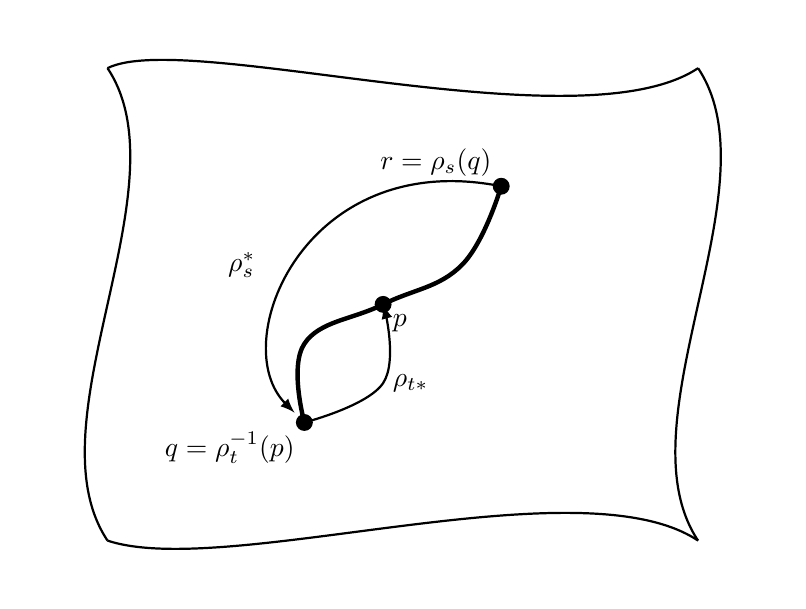
\begin{tikzpicture}



\node at (1,1) {};


\draw [thick] (-6,-4) .. controls (-7,-2.5) and (-5,0.5) .. (-6,2);
\draw [thick] (-6,2) .. controls (-5,2.5) and (0,1) .. (1.5,2);
\draw [thick] (1.5,2) .. controls (2.5,0.5) and (0.5,-2.5) .. (1.5,-4);
\draw [thick] (1.5,-4) .. controls (0,-3) and (-4.5,-4.5) .. (-6,-4);

\node [below left] (p) at (-3.5,-2.5) {$q = \rho_t^{-1}(p)$};
\node [below right] (q) at (-2.5,-1) {$p$};
\node [above left] (r) at (-1,0.5) {$r = \rho_s(q)$};

\node (p') at (-3.5,-2.5) {};
\node (q') at (-2.5,-1) {};
\node (r') at (-1,0.5) {};

\draw [fill = black] (p') circle (0.1);
\draw [fill = black] (q') circle (0.1);
\draw [fill = black] (r') circle (0.1);

\draw [ultra thick]  plot[smooth, tension=.7] coordinates {(p') (-3.5,-1.5) (q') (-1.5,-0.5) (r')};

\draw [thick, -latex] plot[smooth, tension=.7] coordinates { (p') (-2.5,-2) (q') };
\draw [thick, -latex](-1,0.5) .. controls (-3.5,1) and (-4.5,-1.5) .. (p');

\node [left] at (-4,-0.5) {$\rho_s^*$};
\node [right] at (-2.5,-2) {$\rho_{t*}$};

\end{tikzpicture}
		\caption{The series of pullbacks and pushforwards required to `compare' forms in $\bigwedge^p T^*_rM$ to $\bigwedge^p T^*_pM$ so that we can perform a Lie derivative.}
		\label{fig:genLieDeriv}
	\end{figure}\todo{Caption}
Later, we will come across terms such as $\tfrac{d}{dt} \left[ \rho_t^* \omega_t \right]$. To evaluate this, we consider the $t$'s within the bracket to be separate variables, differentiate with respect to each, then evaluate at the point where they both coincide with $t$. Thus
	\begin{align}\label{eq:doubleDerivative}
		\tfrac{d}{dt} \left[ \rho^*_t \omega_t \right] 
		= \left[ \tfrac{\partial}{\partial r} (\rho^*_r \omega_t) \right]|_{r=t} + \left[ \tfrac{\partial}{\partial s} (\rho^*_t \omega_s) \right]|_{s=t}
		= \rho^*_t (\mathcal{L}_{X_t} \omega_t) + \rho^*_t \frac{d \omega_t}{dt}.
	\end{align}

\begin{definition}[Normal bundle]
	Let $M$ be an $n$-dimensional manifold, with $X \subset M$ a $k$-dimensional submanifold. The \textbf{normal bundle} to $X$ in $M$ is the $n$-dimensional manifold
		\begin{align}
			NX \coloneqq \{ (p,v) | p \in X, v \in T_pM / T_pX \}.
		\end{align}
	We can consider the inclusion $X \hookrightarrow NX$, defined by $i_0 : p \mapsto (p,0)$, as well as the usual $i: X \hookrightarrow M$.
\end{definition}

\begin{theorem}[Standard Tubular Neighbourhood Theorem]\label{thm:tubNhood}
	Let $X$ be a submanifold of $M$ with a stricly lower dimension. Then there exists a neighbourhood $U_0$ of $X$ in $NX$ and $U$ of $X$ in $M$ with a diffeomorphism $\phi: U_0 \to U$ such that $\phi \circ i_0 = i$.
\end{theorem}

\begin{definition}[Tubular neighbourhood]
	A neighbourhood $U$ of $X$ in $M$ for which a subset $U_0 \simeq U$ of $NX$ can be found is known as a \textbf{tubular neighbourhood} of $X$.
\end{definition}
	
\begin{remark}
	The name is quite telling. Consider \autoref{fig:tubularNeighbourhood}. The green lines can be thought of as the image of the exponential map of points in the normal bundle of $X$ (the blue line). So long as we follow the flow for a sufficiently small `time', we can use this map to form a bijection between some neighbourhood of $X$ in $NX$, and another neighbourhood of $X$ in $M$. Note, unlike the figure suggests, the flow time need not be constant for all $p \in X$, though there is a \textit{convexity} property for $U_0$, that if $(p,v) \in U_0$, then $(p,\lambda v) \in U_0 \forall \lambda \in [0,1]$.
\end{remark}

\begin{figure}
	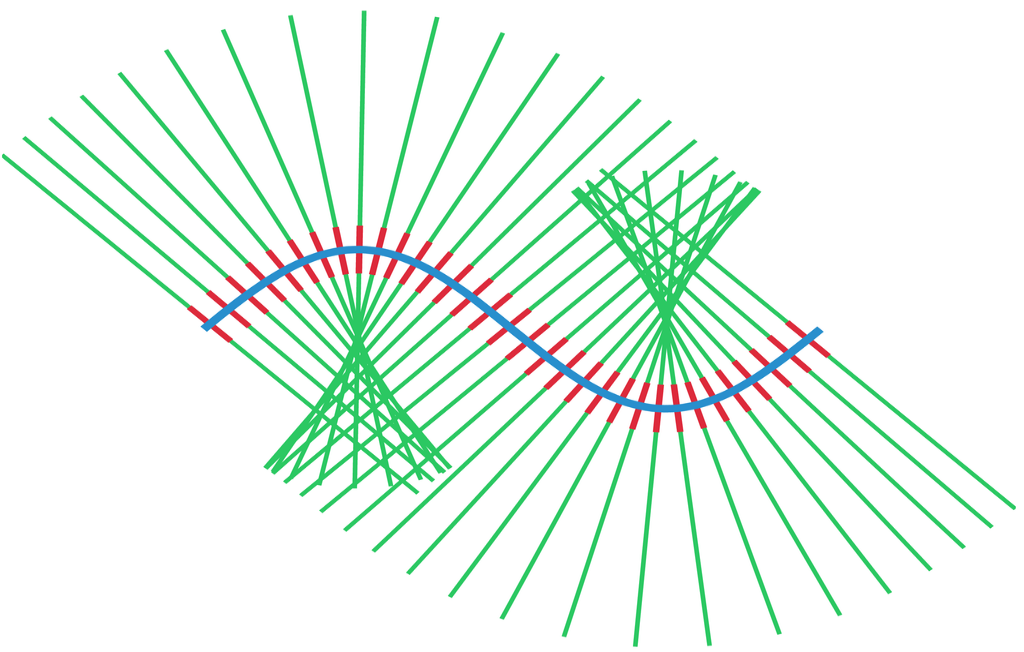
\includegraphics[width=0.8\linewidth]{fig/TubularNeighbourhood}
	\caption{The construction of a tubular neighbourhood using the normal bundle. The `tube', represented by the space swept out by the red lines, can be thought of as either a subset of $NX \supset \{ (p,v) : p \in X, g(v,v) < \epsilon\} $ for some arbitrary Riemannian metric, and $\epsilon >0$. Alternatively, it can be thought of as the subset of $M$ given by $\{ \mathrm{Exp}(v)(p) : (p,v) \in NX \}$. The tubular neighbourhood theorem essentially guarantees that we can take $\epsilon$ to be small enough that the Exp map is a bijection.}\label{fig:tubularNeighbourhood}
\end{figure}

\begin{prop}\label{prop:FuckDeRham}
	Let $U$ be a tubular neighbourhood of $X$. Let $\omega \in \Omega^\ell (U)$ vanish on $X$, i.e. $i^* \omega = 0$. Then $\omega$ is exact, i.e. $\omega = d\mu$ for some $\mu \in \omega^{\ell -1}(U)$. Moreover, we can choose $\mu$ such that $i^* \mu \equiv 0$.
\end{prop}
\begin{proof}
	Let $U_0 \simeq U$ be a neighbourhood of $X$ in $NX$. Consider the family of maps
		\begin{align}
			\rho_t : U_0 \to U_0 ; (p,v) \mapsto (p,tv),
		\end{align}
	where $t \in [0,1]$. This is well defined by the aforementioned convexity of $U_0$. We say that each $\rho_t$ \textit{fixes} $X$, as the image of $X$ under the inclusion $i_0: p \mapsto (p,0)$ is invariant under each $\rho_t$. Naturally $\rho_1 = \mathrm{Id}$, further, $\rho_0 = i_0 \circ \pi_0$, where $\pi_0 : NX \to X$ is the natural projection. We say that the family $\{ \rho_t \}$ is a \textbf{homotopy} from $i_0 \circ \pi_0$ to Id `fixing' $X$. In relation to \autoref{fig:tubularNeighbourhood}, we can consider the action of this as $t$ varies from $1$ to $0$ as retracting the red region onto the blue line. Indeed, $X$ is referred to as a \textbf{deformation retract} of $U$. We can now define the de Rham \textbf{homotopy operator} $Q: \Omega^\ell (U_0) \to \Omega^{\ell -1}(U_0)$ as
		\begin{align}
			Q \omega = \int_0^1 \rho^*_t(\iota_{v_t} \omega ) \mathrm{d}t,
		\end{align}
	where $v_t$ is the time-dependent vector field associated with $\rho_t$. It can be shown that $Q$ satisfies the \textbf{homotopy formula}
		\begin{align}
			dQ + Qd + (i_0 \circ \pi_0)^* = \mathrm{Id} .
		\end{align}
Applying this to the \textit{closed} form $\omega$, and noting that $i_0^* \omega = 0$, we see that $\omega = dQ\omega$, i.e. $Q\omega = \mu$ is a primitive of $\omega$. The existence of $Q$ has thus proved the first claim of the proposition. Our particular choice proves the second, as $\rho_t|_X \equiv \mathrm{Id} \forall t \in [0,1] \Rightarrow v_t|_X \equiv 0$, thus $Q\omega|_X \equiv 0$.
\end{proof}

\subsection{Symplectic Linear Algebra}

\begin{theorem}[Standard Form Theorem]
	Let $V$ be a finite dimensional, real vector space and let $\Omega: V \times V \to \mathbb{R}$ be a skew-symmetric bilinear map, i.e. $(V,\Omega)$ is a symplectic vector space. Then there exists a basis 
		\begin{align}
			V = \mathrm{Span} \{ u_i \}_{i=1}^k \cup \{ e_i \}_{i=1}^n \cup \{ f_i \}_{i=1}^n,
		\end{align}
	which satisfies
		\begin{enumerate}[label = (\roman*)]
			\item $\Omega ( u_i, v ) = 0$, $\forall \, v \in V$.
			\item $\Omega(e_i,e_j) = \Omega(f_i,f_j) = 0$, $\forall \, i,j \in \{1,\ldots, n\}$.
			\item $\Omega(e_i,f_j) = \delta_{ij}$.
		\end{enumerate}
\end{theorem}
\begin{proof}
	The proof is essentially a skew-symmetric adaptation of the Gram-Schmidt process. The $u_i$ are trivial, as we merely need to select \textit{any} basis of $U \coloneqq \{u \in V : \Omega(u,v) = 0 \forall v \in V \}$. Now $\Omega$ is non-degenerate on $V/U \eqqcolon W$.
	
	Let $e_1 \in W/\{0\}$, then there must exist some $\tilde{f}_1 \in W/\{0\}$ such that $\Omega(e_1,\tilde{f}_1)\neq 0$. By linearity, we can rescale $\tilde{f}_1$ to
		\begin{align}
			f_1 \coloneqq \frac{\tilde{f}_1}{\Omega(e_1,\tilde{f}_1)},
		\end{align}
	such that $\Omega(e_1,f_1)=1$ as desired. Let $W_1 \coloneqq \mathrm{Span} \{e_1,f_1\}$. We can then repeat this procedure for $W/W_1$ to find $e_2,f_2$ and so on, each satisfying $\Omega(e_i,f_i) = 1$. But, how do we guarantee that $\Omega(e_i,f_j) = 0$ for distinct $i,j$? Thinking of $W/W_1$ as a modulo relation, we simply need to show that, $\forall w \in W$, there exists $v \in W^\Omega_1 \coloneqq \{ x \in W : \Omega(x,y) = 0 \forall y \in W_1\}$ such that $w \sim v$. In other words $w-v = a e_1 + b f_1$, for some constant $a,b$. Acting on either side of this with $\Omega(e_1, \cdot)$ and $\Omega(f_1, \cdot)$ tells us that this is satisfied only if $a = - \Omega(f_1,w)$ and $b = - \Omega(e_1,w)$, thus
		\begin{align}
			v = w + \Omega(f_1, w) e_1 - \Omega(e_1 ,w) f_1.
		\end{align}
	To verify this is still in $W_1^\Omega$, we must then consider $\Omega(v,\tilde{w})$ for some arbitrary $\tilde{w} \in W_1$. Writing the general form of $\tilde{w}$ we see
		\begin{align}
			\begin{split}
				\Omega(v,ce_1 + d f_1) = \, &c \left[ \cancel{\Omega(w,e_1)} + \Omega(f_1,w) \Omega(e_1,e_1) - \cancel{\Omega(e_1,w) \Omega(f_1,e_1)} \right] \\
									   + &\, d \left[ \cancel{\Omega(w,f_1)} + \cancel{\Omega(f_1,w) \Omega(e_1,f_1)} - \Omega(e_1,w) \Omega(f_1,f_1) \right] \\
									   = &\, 0.
			\end{split}
		\end{align}
	Thus, indeed $W = W_1 \oplus W_1^\Omega$ and we can repeat this to show that all distinct $e_i$ and $f_j$ are `orthogonal' with respect to $\Omega$. An alternative justification is that, if my initial choice of $\tilde{e}_2, \tilde{f}_2$ are not orthogonal to both $e_1, f_1$, I can translate them by a combination \textit{of} $e_1, f_1$ such that resulting are orthogonal to both, then rescale similar to before.
\end{proof}

\begin{definition}[Rank]
	The rank of $\Omega$ is $n = \tfrac{1}{2} \left(\mathrm{Dim } V - \mathrm{Dim } U \right)$
\end{definition}

\begin{remark}
	If we endow $V$ with a Euclidean metric such that the above basis is orthonormal, then $\Omega$ has a (block) matrix representation as
		\begin{align}
			\Omega = \begin{pmatrix}
				0 & 0 & 0 \\ 0 & 0 & \mathds{1}_n \\ 0 & -\mathds{1}_n & 0
			\end{pmatrix}.
		\end{align}
\end{remark}

\begin{definition}[Symplectic subspace]
	$W \subset V$ is a \textbf{symplectic subspace} of $V$ if $\Omega|_{W \times W}$ is non-degenerate
\end{definition}
\begin{definition}[Isotropic subspace]
	$W \subset V$ is an \textbf{isotropic subspace} if $\Omega|_{W \times W} \equiv 0$. I.e. in standard form, $W = \mathrm{Span} \{e_i : {i \in I \subset \{1, \cdots n\}}\}$ or $\mathrm{Span} \{f_i : {i \in I \subset \{1, \cdots n\}}\}$
\end{definition}
\begin{definition}[Lagrangian subspace]
	A \textbf{Lagrangian subspace} is a maximal isotropic subspace.
\end{definition}

\begin{definition}[Symplectomorphism]
	A \textbf{symplectomorphism} between symplectic vector spaces $(V,\Omega)$ and $(V',\Omega')$ is an isomorphism $\phi : V \to V'$ such that $\Omega \equiv \phi^*\Omega': (u,v) \mapsto \Omega'(\phi(u),\phi(v))$.
\end{definition}
\begin{remark}
	For non-degenerate symplectic vector spaces, the standard form theorem essentially states that they are symplectomorphic to $( \mathbb{R}^{2n},\Omega_0 )$, where $\Omega_0$ is the standard, non-degenerate symplectic form on $\mathbb{R}^{2n}$.

\end{remark}

\subsubsection{Aside: Nuances of Symplectic Linear Algebra}

\todo[inline]{Discuss. In particular, mention musical iso's, similarities and differences compared to metrics. Little bit of $ Sp(2n) $}
	
\subsection{Symplectic Manifolds}

\begin{definition}[Symplectic form]
	A \textbf{symplectic form} $\omega$ on a differential manifold $M$ is a 2-form which is \textit{closed} ($d\omega = 0$) and \textit{non-degenerate} ($\omega^n \coloneqq \omega \wedge \cdots \wedge \omega \neq 0$).
\end{definition}
\begin{remark}
	As $\omega|_p$ is be non-degenerate $\forall p \in M$, $T_pM$ must be even-dimensional, thus so too must $M$.
\end{remark}

\begin{example}
	The standard symplectic manifold is $\left( \mathbb{R}^{2n},\omega_0 \right)$, where, using the standard chart $(x^1, \ldots, x^n, y^1, \ldots, y^n)$
		\begin{align}
			\omega_0 \coloneqq \sum_{i=1}^n dx^i \wedge dy^i.
		\end{align}
\end{example}

\begin{example}
	Consider $S^2 \subset \mathbb{R}^3$. For $\mathbf{p} \in S^2$, $T_pS^2 \cong \{ \mathbf{v} \in \mathbb{R}^3 : v \cdot p = 0\}$, thus ${\mathbf{u} \times \mathbf{v}} \propto \mathbf{p}$, $\forall \mathbf{u}, \mathbf{v} \in T_pS^2$. We can use this to define a symplectic map on $T_pS^2$, 
		\begin{align}
			\Omega(\mathbf{u},\mathbf{v}) \coloneqq \mathbf{p} \cdot (\mathbf{u}\times\mathbf{v}) \eqqcolon \omega|_{\mathbf{p}}.
		\end{align}
	A 2-form on a 2-dimensional manifold is necessarily closed, and ${\omega|_\mathbf{p}(\mathbf{u},\mathbf{u}\times \mathbf{p}) \neq 0}$, thus $\omega$ is non-degenerate.
\end{example}

\begin{definition}[Notions of equivalence for symplectic manifolds]
	Let $(M,\omega)$ and $(M,\omega')$ be two symplectic manifolds, they are
		\begin{enumerate}[label=(\roman*)]
			\item \textbf{Symplectomorphic} if there exists a diffeomorphism $ \phi: M \to M' $ such that $\phi^* \omega' \equiv \omega$. Then $\phi$ is called a \textbf{symplectomorphism}.
			\item \textbf{Strongly isotopic} if there exists a smooth map $\rho : M \times [0,1] \to M$ such that $\rho_0 \equiv \mathrm{Id}$, and $\rho_1^* \omega' \equiv \omega$. The family of diffeomorphisms ${\{ \rho_t : M \to M \}}$ is an \textbf{isotopy}\footnote{The condition that $\rho_1$ is a symplectomorphism is not part of the definition of an isotopy, but the rest is.}.
			\item \textbf{Deformation equivalent} if there is a smooth family of symplectic forms $\omega_t$ such that $\omega_0 \equiv \omega$ and $\omega_1 \equiv \omega'$.
			\item \textbf{Isotopic} if they are deformation equivalent and the cohomology classes $[\omega_t]$ are independent of $t$.
		\end{enumerate}
\end{definition}
\begin{remark}
	How do these notions relate to each other?
		\begin{enumerate}[label = (\Roman*)]
			\item Strongly isotopic $\Rightarrow$ symplectomorphic, as $\rho_1$ is a symplectomorphism.
			\item As the name suggests, strongly isotopic $\Rightarrow$ isotopic, this is because, for a {diffeomorphism} $\phi$, $[\phi^* \omega] = [\omega]$, thus $\omega_t := \rho_t^* \omega'$ is a deformation of constant cohomology class.
			\item It turns out (Moser) that isotopic + $M$ compact $\Rightarrow$ strongly isotopic.
		\end{enumerate}
\end{remark}
\begin{prop}[Moser's trick]
	Let $(M,\omega)$, $(M,\omega')$ be isotopic. Suppose there exists an isotopy $\rho: M \times \mathbb{R} \to M$ such that $\rho_t^* \omega_t = \omega$. Let
		\begin{align}
			\nu_t \coloneqq \frac{d\rho_t}{dt} \circ \rho_t^{-1}.
		\end{align}
	Then
		\begin{align}
			\frac{d}{dt}(\rho^*_t \omega_t) = 0 = \rho^*_t (\mathcal{L}_{\nu_t} \omega_t + \frac{d \omega_t}{dt}).
		\end{align}
	Thus
		\begin{align}\label{eq:differentialMoser}
			\mathcal{L}_{v_t} \omega_t + \frac{d \omega_t}{dt} = 0.
		\end{align}
\end{prop}

\begin{theorem}[Moser Theorem - Version I]
	Let $M$ be compact and let $\omega_0$, $\omega_1$ be symplectic forms on $M$ with the same cohomology class, $[\omega_0] = [\omega_1]$. Further, assume that $\omega_t \coloneqq (1-t) \omega_0 + t \omega_1$ is symplectic $\forall t \in [0,1]$. \textbf{Then}, there exists an isotopy $\rho : M \times \mathbb{R} \to M$ such that $\rho^*_t \omega_t \equiv \omega_0$ $\forall t \in [0,1]$.
\end{theorem}
\begin{proof}
	First we see that $\tfrac{d}{dt}\omega_t = \omega_1 - \omega_0$ is exact, thus is equal to $d \mu_t$ for some family of 1-forms $\mu_t$. Thus, substituting our definition of $\omega_t$ into \eqref{eq:differentialMoser}, applying Cartan's magic formula \eqref{eq:CartanMagic}, means that we have a solution if
		\begin{align}
			\iota_{\nu_t} \omega_t + \mu_t = 0.
		\end{align}
	This is \textbf{Moser's equation}. As $\omega_t|_p$ is non-degenerate $\forall t \in [0,1], p \in M$, we can solve this pointwise for $\nu_t|_p$.
\end{proof}

\begin{theorem}[Moser Theorem - Version II]
	Let $M$ be compact with symplectic forms $\omega_0$ and $\omega_1$. Let $\omega_t, t\in [0,1]$ be a smooth family of symplectic forms joining $\omega_0$ to $\omega_1$ such that $[\omega_t] = [\omega_{t'}], \forall t,t' \in [0,1]$.	\textbf{Then}, there exists an isotopy $\rho: M\times\mathbb{R} \to M$ such that $\rho^*_t \omega_t = \omega_0, \forall t \in [0,1]$.
\end{theorem}

\begin{proof}
	Similarly to before, we have that $\tfrac{d}{dt} \omega_t$ is exact. Let $\mu_t$ be its primitive 1-form, this is a smooth family. From here, we can again set up and solve the Moser equation for the desired isotopy.
\end{proof}

\begin{theorem}[Moser Theorem - Relative Version]
	Let $M$ be a manifold with compact submanifold $X$.	Let $\omega_0$ and $\omega_1$ be symplectic forms on $M$ such that $\omega_0|_X \equiv \omega_1|_X$. \textbf{Then}, there exist neighbourhoods $U_0,U_1$ of $X$ in $M$ and a diffeomorphism $\phi: U_0 \to U_1$ such that $\phi^* \omega_1|_X \equiv \omega_0|_X$ and the following diagram commutes, where $i: X \hookrightarrow M$ is the inclusion map.
	\begin{center}
		\begin{tikzpicture}

	\node (v1) at (-2.5,1.5) {$U_0$};
	\node (v2) at (0.5,1.5) {$U_1$};
	\draw [->]  (v1) edge (v2);
	\node at (-1,2) {$\phi$};
	\node (v3) at (-1,-0.5) {$X$};
	\draw [->]  (v3) edge  node [left]  {$i$} (v1);
	\draw [->]   (v3) edge node [right] {$i$} (v2);

%\node at (0.5,-0.5) {commutes.};
\end{tikzpicture}
	\end{center}
\end{theorem}
\begin{proof}
	Let $U_0$ be a \textit{tubular} neighbourhood of $X$. As both $\omega_{\nicefrac{0}{1}}$ are closed on $U_0$, and $\omega_1 - \omega_0$ vanishes on $X$, we can invoke proposition \ref{prop:FuckDeRham}, and find a $1$-form $\mu$ on $U_0$ such that $\omega_1 = \omega_0 + d \mu$, and $\mu|_X \equiv 0$. We thus have a family of symplectic forms $\omega_t = \omega_0 + td\mu$ connecting $\omega_0$ to $\omega_1$.\footnote{Apparently the $\omega_t$ will always be symplectic on some `sufficiently small' tubular neighbourhood of $X$.} We now proceed similarly to before, substituting $\omega_t$ into \eqref{eq:differentialMoser} to get
		\begin{align}
			\iota_{\nu_t} \omega_t + \mu = 0
		\end{align}
Given a sufficiently small $U_0$, the resulting $\nu_t$ can be integrated to an isotopy $\rho: U_0 \times [0,1] \to M$ satisfying the desired $\rho_t^* \omega_t = \omega_0$. Moreover, the fact that we can take $\mu|_X \equiv 0$ implies that $\nu_t|_X \equiv 0$, hence $\rho_t|_X \equiv \mathrm{Id}$. The symplectomorphism required to complete the theorem is then $\rho_1 : U_0 \to U_1 \coloneqq \rho_1(U_0)$.
\end{proof}

\begin{theorem}[Darboux]
	Let $(M,\omega)$ be a symplectic manifold. For any $p \in M$, we can find a chart $(U, \phi), \phi: q \mapsto (x^i, y^i)$ such that
		\begin{align}
			\omega|_U = \sum_{i=1}^{n} dx^i \wedge dy^i.
		\end{align}		 
\end{theorem}
\begin{proof}
	As $\omega|_p$ is non degenerate, we can use the standard form theorem to construct a basis $\{ d\tilde{x}^i, d\tilde{y}^i \}$ of $T^*_pM$ such that $\omega|_p = \sum_i d\tilde{x}^i\wedge d\tilde{y}^i$. We can then `exponentiate this slightly' to a symplectic form $\tilde{\omega} = \tilde{\phi}^* \omega_0$ on some chart $(\tilde{U}, \tilde{\phi})$ around $p$. As $\omega$ and $\tilde{\omega}$ agree on the compact submanifold $\{p\} \subset X$, assuming $\tilde{U}$ to be sufficiently small, there is a symplectomorphism $\psi$ from $(U,\omega)$ to $(\tilde{U},\tilde{\omega})$, for some neighbourhood $U$ of $p$. Finally $\omega = \psi^* \phi^* \omega_0 = (\tilde{\phi} \circ \psi)^* \omega_0$, thus $\phi \coloneqq \tilde{\phi} \circ \psi$ is the required map from $U \to \mathbb{R}^{2n}$.
\end{proof}

\subsection{The Cotangent Bundle}

\paragraph{} The cotangent bundle is a motivating example for many of the interesting features of symplectic geometry, arguably owing to its role in classical mechanics.

\begin{definition}[Phase space and configuration space]
	If $X$ is a manifold and $M = T^*X$, then we can call $X$ the \textbf{configuration space} corresponding to the \textbf{phase space} $M$.
\end{definition}
\begin{remark}
	Given a chart $\left(U,(x^i)\right)$ on $X$, we can define a compatible chart $\left( T^*U,(x^i \xi_i ) \right)$ on $M$. Abstractly speaking, the chart $(T^*U, \Phi)$ on $M$ is compatible with $(U,\phi)$ if ${P \circ \Phi \equiv \phi \circ \pi}$, where $P : \mathbb{R}^{2n} \to \mathbb{R}^n$ is the projection $(x^1,\cdots, x^{2n}) \mapsto (x^1, \cdots x^n)$ and $\pi: T^*U \to U$ is the canonical projection. 
\end{remark}

\begin{definition}[Tautological form \& canonical symplectic form]
	Given a configuration space $M$ for the phase space $X$, the \textbf{tautological form} is a $1$-form on $M$ defined, for $p = (x,\xi) \in M$, by
		\begin{align}\label{eq:tautForm}
			\alpha = \pi^* \xi.
		\end{align}
	Given a set of local coordinates $(x^i , \xi_i)$, we can equivalently write this as 
		\begin{align}
			\alpha = \xi_i dx^i.
		\end{align}
	We can then define the \textbf{canonical symplectic form} both globally and locally
		\begin{align}
			\omega \coloneqq - d\alpha = dx^i \wedge d\xi_i.
		\end{align}
\end{definition}\todo{Verify coincidence of definitions?}

\begin{prop}[Naturality of $\alpha$ and $\omega$]
	Let $X_1$, $X_2$ be the phase spaces of two configuration spaces $M_1$, $M_2$. Let $\phi: X_1 \to X_2$ be a diffeomorphism, and let $\phi_\# : M_1 \to M_2$ be its \textbf{lift}, defined by
		\begin{align}
			\phi_\#: (x, \xi) \mapsto \big(\phi(x), \phi_*|_x \xi|_x \big).
		\end{align}
	Then $\phi_\#$ is a symplectomorphism from $(M_1,\omega_1)$ to $(M_2,\omega_2)$, where $\omega_i$ are the canonical symplectic forms.
\end{prop}
\begin{proof}
	As $\phi^*_\#$ commutes with $d$, it is sufficient to show that $\phi^*_\# \alpha_2 = \alpha_1$. From \eqref{eq:tautForm}, we then have
		\begin{align}
			(\phi^*_\# \alpha_2)
			= \phi^*_\# \pi_2^* \xi_2
			= (\pi_2 \circ \phi_\# )^* \phi_* \xi.
		\end{align}
	Note that $\pi_2 \circ \phi_\# (x,\xi) = \phi(x) = \phi \circ \pi_1 (x,\xi)$, thus
		\begin{align}
			\phi^*_\# \alpha_2 = (\phi \circ \pi_1)^* \phi_* \xi = \pi_1^* \phi^* \phi_* \xi = \pi_1^* \xi.
		\end{align}
\end{proof}
\begin{remark}
	Note that whilst all diffeomorphisms on the phase spaces lift to symplectomorphisms on the configuration spaces, the converse fails to hold in general. See below the correct statement.
\end{remark}

\begin{prop}
	Let $g: T^*X \to T^*X$ be a symplectomorphism. Then $g = \phi_\#$ for some diffeomorphism $\phi$ iff $g^* \alpha = \alpha$.
\end{prop}
\begin{proof}
	\todo[inline]{Do Proof}
\end{proof}

\begin{remark}
	Let $\mu \in \Omega^1(X)$. We can consider $(x,\mu|_x)$ as a subspace of $M$, specifically it is the \textit{section} (i.e. smooth preimage of $X$ w.r.t. $\pi$) given by the map $S_\mu: X \to M$. We can use this to justify $\alpha$'s title of `tautological' via the following result.
\end{remark}
\begin{prop}\label{prop:tautologicality}
	$S_\mu^* \alpha = \mu$.
\end{prop}
\begin{proof}
	$S_\mu^* \alpha = S_\mu^* \pi^* \mu = (\underbrace{\pi \circ S_\mu}_{\equiv \mathrm{Id}})^* \mu = \mu$
\end{proof}

\section{Lagrangian Submanifolds}

\begin{definition}[Lagrangian submanifold]
	A submanifold $L$ of a symplectic manifold $(M,\omega)$ is a \textbf{Lagrangian submanifold} if $T_pL$ is a Lagrangian subspace of $T_pM$, $\forall p \in L$. Equivalently, if $i: L \hookrightarrow M$ is the inclusion map, then $i^*\omega \equiv 0$, and $\mathrm{Dim}(L) = \tfrac{1}{2} \mathrm{Dim}(M)$.
\end{definition}
\begin{remark}
	If $\mathrm{Dim}(M) = 2$, then \textit{all} 1D submanifolds of $M$ are Lagrangian, as any symplectic form $\omega|_p$ must vanish on a 1D vector space.
\end{remark}

\subsection{Lagrangian Submanifolds of \titlemaths{T^*X}}

\begin{prop}
	Let $S_\mu$ be as before in proposition \autoref{prop:tautologicality}, and let $X_\mu = \mathrm{Img}(S_\mu)$. Then $X_\mu$ is a $\mathrm{Dim}(X) = \tfrac{1}{2}\mathrm{Dim}(M)$ dimensional submanifold of $M$. $X_\mu$ is Lagrangian if $\mu$ is closed on $X$.
\end{prop}
\begin{proof}
	$X_\mu$ is Lagrangian if $S^*_\mu \omega$ vanishes, thus
		\begin{align}
			\begin{split}
				S^*_\mu \omega 
				&= S^*_\mu (-d\alpha) = -d \left( S^*_\mu \alpha \right) \\
				&= - d \mu = 0.
			\end{split}
		\end{align}
\end{proof}
\begin{remark}
	In particular, if $\mu$ is \textit{exact}, i.e. $\mu = dh$ for some $h \in C^\infty(X)$, then $X_{dh}$ is always Lagrangian. We then call $h$ the \textbf{generating function} of $X_\mu$.
\end{remark}

\begin{definition}[Conormal space \& conormal bundle]
	Let $S$ be a $k$-dimensional submanifold of the $n$-dimensional manifold $X$. The \textbf{conormal space} of $S$ at $x \in S$ is defined as
		\begin{align}
			N_x^*S \coloneqq \{ \xi \in T^*_xX : i_0^*|_x \xi = 0 \},
		\end{align}
	where $i_0 : S \hookrightarrow X$ is the inclusion map.
	The \textbf{conormal bundle} is simply the smooth manifold obtained by taking the disjoint union of all conormal spaces
		\begin{align}
			N^*S \coloneqq \bigsqcup_{x \in S} N^*_xS = \{ (x,\xi) : x \in S, \xi \in N_x^*S\}.
		\end{align}
\end{definition}

\begin{example}
	\begin{enumerate}[label=(\roman*)]
		\item If $S = \{x\}$, then $T_xS = \{ 0 \}$, thus $N^*_xS = N^*S = T^*_xX$.
		
		\item If $S = X$, then only the zero covector $0 \in T^*_xX$ vanishes, thus $N^*S = \{ (x,0) : x \in X \}$ is the zero section $S_0(X)$.	
	\end{enumerate}
\end{example}
\begin{remark}
In both cases, $N^*S$ is an $n$-dimensional submanifold of $T^*X$. It turns out that this is \textit{always} the case.
\end{remark}

\begin{prop}
	The conormal bundle $N^*S$ is a Lagrangian submanifold of $M$.
\end{prop}
\begin{proof}
	If we think of the pullback of the inclusion from $S$ to $X$ as (specifically) ${i_0^*|_x: T_x^*X \to T_x^*S}$, then $N^*_xS = \mathrm{Ker}(i^*_0|_x)$. The map is surjective, thus $\mathrm{Dim}(N^*_xS) = n-k$. Hence, $N^*S$ is a rank $n-k$ vector bundle over the $k$-dimensional base space $S$, which has dimension $k + (n-k) = n$.
	
	Next, to show that $\omega$ vanishes on $N^*S$, it suffices to prove $i^* \alpha$ vanishes, where $i: N^*S \hookrightarrow T^*X$. Consider the commutative diagram:
		\begin{center}
			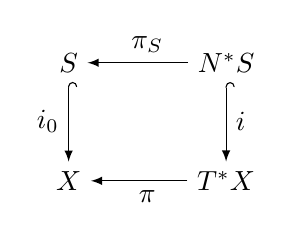
\begin{tikzpicture}

\node (v1) at (-2,1.5) {$S$};
\node (v3) at (0,1.5) {$N^*S$};
\node (v2) at (-2,0) {$X$};
\node (v4) at (0,0) {$T^*X$};

\draw  [right hook -latex] (v1) edge (v2);

\node [left] at (-2,0.75) {$i_0$};
\node [right] at (-0,0.75) {$i$};
\node [above] at (-1,1.5) {$\pi_S$};
\node [below] at (-1,0) {$\pi$};

\draw [-latex] (v3) edge (v1);
\draw [-latex] (v4) edge (v2);
\draw [right hook -latex] (v3) edge (v4);

\end{tikzpicture}
		\end{center}
	From this we have
		\begin{align}
			i^*\alpha|_{(x,\xi)} = i^* ( \pi^*|_x \xi ) = (\pi \circ i)^*|_x \, \xi = (i_0 \circ \pi_S )^*|_x \, \xi = \pi_S^* ( i_0^*|_x \xi) = 0.
		\end{align}
\end{proof}

\subsection{Lagrangians \& Symplectomorphisms}

\begin{definition}[(Twisted) Product form]
	Let $(M_1,\omega_1)$, $(M_2, \omega_2)$ be symplectic manifolds. Further, let $p_i: M_1 \times M_2 \to M_i$ be the projection from the product space onto each factor. Then the \textbf{product form} is a $2$-form on $M_1 \times M_2$ defined by
		\begin{align}
			\omega \coloneqq p_1^* \omega_1 + p_2^* \omega_2.
		\end{align}
	The \textbf{twisted product form} is similarly defined by
		\begin{align}
			\tilde{\omega} \coloneqq p_1^* \omega_1 - p_2^* \omega_2.
		\end{align}
\end{definition}
\begin{remark}
	The (twisted) product form is symplectic. In fact, $\lambda_1 p_1^* \omega_1 + \lambda_2 p_2^* \omega_2$ is symplectic $\forall \lambda_1, \lambda_2 \in \mathbb{R}/\{0\}$.
\end{remark}

\begin{prop}
	Let $f: M_1 \to M_2$ be a diffeomorphism, and let ${T_f \coloneqq \{ (p_1,f(p_1)) : p_1 \in M_1 \} }$ be the \textbf{graph} of $f$. Then $f$ is a symplectomorphism iff $T_f$ is a Lagrangian submanifold of $(M_1 \times M_2, \tilde{\omega})$.
\end{prop}
\begin{proof}
	Let $\gamma_f: M_1 \hookrightarrow M_1 \times M_2; p_1 \mapsto (p_1, f(p_1))$, so $T_f = \mathrm{Img} ( \gamma_f )$. $T_f$ is Lagrangian iff $\gamma^*_f \tilde{\omega} = 0$. Computing this, we see
		\begin{align}
			\gamma^*_f \tilde{\omega} = \gamma^*_f p^*_1 \omega_1 - \gamma^*_f p^*_2 \omega_2 = (p_1 \circ \gamma_f)^* \omega_1 - (p_2 \circ \gamma_f)^* \omega_2.
		\end{align}
	Whence, as $p_1 \circ \gamma_f = \mathrm{Id}_{M_1}$ and $p_2 \circ \gamma_f  = f$, the vanishing condition is
		\begin{align}
			\omega_1 - f^* \omega_2 = 0,
		\end{align}
	i.e. that $f^*\omega_2 = \omega_1, \Rightarrow$ $f$ is a symplectomorphism.
\end{proof}

\begin{example}
	If the $M_i = T^*X_i$ are cotangent bundles, then $M_1 \times M_2 \simeq T^*(X_1 \times X_2)$ is itself a cotangent bundle. Unfortunately, the canonical symplectic form $\omega$ on $M_1 \times M_2$ is the standard product form, \textit{not} the twisted product form. However, we can define it relatively easily. Consider the \textbf{involution}
		\begin{align}
			\begin{split}
				\sigma: M_1 \times M_2 &\to M_1 \times M_2, \\
						(x,\xi, y, \eta) &\mapsto (x, \xi, y, -\eta).
			\end{split}
		\end{align}
	It can then be verified that $\sigma^* \omega = \tilde{\omega}$ and $\sigma^* \tilde{\omega} = \omega$, i.e. $\sigma$ is a symplectomorphism $(M_1 \times M_2, \omega) \leftrightarrow (M_1\times M_2, \tilde{\omega})$.
	
From here it is relatively straightfowards to find a family of symplectomorphisms between $M_1$ and $M_2$. Recall that a closed form $\mu$ on $X$ defines a Lagrangian submanifold $X_\mu \subset M$. Thus if we define any function $h \in C^\infty(X_1 \times X_2)$, then $X_{dh} = (x_1, dh_{x_1}, x_2, dh_{x_2})$, where 
	\begin{align}\label{eq:splitGenFunc}
		dh = p_1^* dh_{x_1} + p_2^* dh_{x_2}, 
	\end{align}
is a Lagrangian submanifold of $(M_1 \times M_2,\omega)$. We then use the involution to define $\mathcal{L}^\sigma \coloneqq \sigma(X_{dh})$, which is a Lagrangian submanifold of $(M_1 \times M_2,\tilde{\omega})$.

We now work locally. For convinence, we shall relabel $x_1$ and $x_2$ as $x$ and $y$ respectively. The coordinates of $\mathcal{L}^\sigma$ are thus
	\begin{align}
		\mathcal{L}^\sigma = \left\{ \left(x^i, \tfrac{\partial h}{\partial x^i}, y^i, - \tfrac{\partial h}{\partial y^i} \right) \right\}.
	\end{align}
If $\mathcal{L}^\sigma = T_f$ for some diffeomorphism $f: M_1 \to M_2$, then $f$ is a symplectomorphism.
So long as the implicit function theorem raises no objections, we can find a set of functions $\tilde{y}^i(x,\xi)$ such that $\tfrac{\partial h}{\partial x^i}(x,\tilde{y}(x,\xi)) = \xi_i$. Using these we can define another set of functions
	\begin{align}
		\tilde{\eta}_i(x,\xi) = - \tfrac{\partial h}{\partial y^i}\big(x, \tilde{y}(x,\xi)\big),
	\end{align}
such that the map $f:(x,\xi) \mapsto (\tilde{y}(x,\xi), \tilde{\eta}(x,\xi))$ is the desired symplectomorphism, which was say is \textbf{generated} by $h$.
\end{example}

\begin{prop}
	Let $f \in C^\infty(X\times X)$ generate the symplectomorphism $\phi: M \to M$. Then there is a one-to-one correspondence between fixed points $p \in M$ s.t. $\phi(p) = p$, and critical points of the function $\psi \in C^\infty(X), \psi(x) = f(x,x)$.
\end{prop}
\begin{proof}
	Critical points of $\psi$ are the subset of the points $\{ (x,y) \in X \times X : df|_{(x,y)} \equiv 0 \}$ where $x=y=x_0$. Similarly to \eqref{eq:doubleDerivative}, we can evaluate the derivative of $\psi$ at any point $x_0$ as
		\begin{align}
			\begin{split}
				d \psi|_{x_0} &= df(x,x_0))|_{x=x_0} + df(x_0,y)|_{y=x_0},\\
							  &= df_x|_{x_0} + df_y|_{x_0},
			\end{split}
		\end{align}
	where the $df_x$ and $df_y$ are defined in the same way as \eqref{eq:splitGenFunc}. Recall then that the symplectomorphism generated by $f$ satisfies
		\begin{align}\label{eq:fixedPoints}
			\phi(x, df_x) = (y, -df_y).
		\end{align}
	If $x_0$ is a critical point of $\psi$, then $df_x|_{x_0} = -df_y|_{x_0}$. Substituting this into \eqref{eq:fixedPoints} give the desired result.
\end{proof}
\begin{remark}
	If we can find a function $f^{(N)} \in C^\infty(X \times X)$ generating $\phi^N = \phi \circ \cdots \circ \phi$ for some $N$, then we can generalise this result to \textit{periodic} points of $\phi$ (invariant points of $\phi^N$).
\end{remark}

\begin{prop}
	Let $f \in C^\infty(X \times X)$ generate the symplectomorphism $\phi$. If $ \forall (x,y) \in X \times X$, the map $F_{x,y} \in  C^\infty(X^N)$ defined by
		\begin{align}
			F_{x,y}(z_i) = f(x,z_1) + \sum_{i=1}^{N-1} f(z_i, z_{i+1}) + f(z_N, y)
		\end{align}
	has a \textit{unique} critical point $(\tilde{z}_i)(x,y) \in X^N$, then the map
		\begin{align}
			f^{(N)}(x,y) \coloneqq F_{x,y}(\tilde{z}_i(x,y))
		\end{align}
	is a generating function of $\phi^N$.
\end{prop}
\textbf{Proof Omitted.}

\begin{theorem}[Poincar\' e's Last Geometric Thoerem - {[Birkhoff, 1913]} ]
	Let $\phi: A \to A$ be an area-preserving diffeomorphism such that $\phi$ preserves boundary components and twists them in opposite directions. Then $\phi$ has at least 2 fixed points.
\end{theorem}

\subsection{Fixed Points via Lagrangian Submanifolds}

\begin{theorem}[Lagrangian Neighbourhood Theorem - {[Weinstein 1]}]\label{thm:Weinstein1}
	Let $(M, \omega)$ be a symplectic manifold with a \textit{compact} Lagrangian submanifold $X$. Let $\omega_0$ be the canonical symplectic form on $T^*X$. Further define
		\begin{subequations}\begin{align}
			i_0: &X \hookrightarrow T^*X,  &\mathrm{(embedding as zero section)},\\
			i: &X \hookrightarrow M,  &\mathrm{(embedding by inclusion)}.
		\end{align}\end{subequations}
	\textbf{Then}, there exists neighbourhoods of $X$, $U_0 \subset T^*X$ and $U \subset M$ such that the following diagram commutes
		\begin{center}
			\usetikzlibrary{arrows}
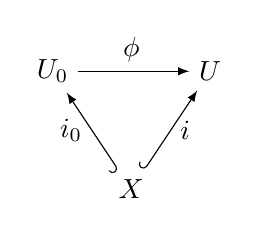
\begin{tikzpicture}

\node (v3) at (-1,1) {$U_0$};
\node (v2) at (1,1) {$U$};
\node (v1) at (0,-0.5) {$X$};

\node [left] at (-0.5,0.25) {$i_0$};
\node [right] at (0.5,0.25) {$i$};

\draw [-latex] (v3) edge (v2);
\draw[right hook -latex] (v1) edge (v2);
\draw [right hook -latex]  (v1) edge (v3);

\node [above] at (0,1) {$\phi$};

\end{tikzpicture}
		\end{center}
	and $\phi^* \omega = \omega_0$.
\end{theorem}

\begin{theorem}[{[Weinstein 2]}]\label{thm:Weinstein2}
	Let $M$ be a $2n$ dimensional manifold with compact $n$ dimensional submanifold $X$. Let $i: X \hookrightarrow M$ be the inclusion map. Let $\omega_0$, $\omega_1$ be symplectic forms on $M$ such that $X$ is Lagrangian in $(M,\omega_{\nicefrac{0}{1}})$. \textbf{Then}, there exists neighbourhoods $U_0$, $U_1$ of $X$ in $M$ with a diffeomorphism $\rho: U_0 \to U_1$ such that $\rho|_X \equiv \mathrm{Id}$, and $\rho^* \omega_1 \equiv \omega_0$.
\end{theorem}

\begin{proof}[Proof of \autoref{thm:Weinstein1}]
	Firstly, note that for any non-degenerate symplectic vector space $V$ with Lagrangian subspace $L$, we can define a non-degenerate bilinear form
		\begin{align} \begin{split}
			\Omega^1 : V/L \times L &\to \mathbb{R}, \\
				\left([v],u\right) &\mapsto \Omega(v,u).
		\end{split} \end{align}
	This induces an isomorphism $\flat: V / L \congto L^*$, by $ [v] \mapsto \left( [v]_\flat: u \mapsto \Omega^1\left([v],u\right) \right)$. Noting that $T_pX$ is Lagrangian in $T_pM$, and $T_pM / T_pX = N_pX$, we thus have an isomorphism $\flat: N_pX \congto T^*_pX$, which induces a diffeomorphism $\varphi: NX \simto T^*X$. Thus we can invoke \autoref{thm:tubNhood} to find a neighbourhood $\tilde{U}_0$ of $X$ in $NX$ that is diffeomorphic to some $\tilde{U}$ of $X$ in $M$. Let $\psi: \tilde{U}_0 \simto \tilde{U}$, then on $NX$ we can pullback both the canonical symplectic form $\tilde{\omega_0} \coloneqq \varphi^* \omega_0$, as well as $\tilde{\omega} \coloneqq \psi^* \omega$. Naturally $X$ is Lagrangian in $NX$ with respect to both, the latter due to the fact that $i_0^* \tilde{\omega} = (\psi \circ i_0)^* \omega = i^* \omega$. By \autoref{thm:Weinstein2}, we then have a diffeomorphism $\rho: \tilde{U}_0 \simto \tilde{U}_1$ such that $\rho^* \tilde{\omega} = \omega_0$. Shrinking $\tilde{U}_1$ until it is within the domain of $\psi$, the diffeomorphism $\phi \coloneqq \psi \circ \rho \circ \varphi^{-1}$ between $U_0 \coloneqq \varphi^{-1}(\tilde{U}_0)$ and $U \coloneqq \psi(\tilde{U}_1)$ has the desired properties. In essence, for appropriately reduced neighbourhoods, the following diagram commutes
		\begin{center}
			\usetikzlibrary{arrows}
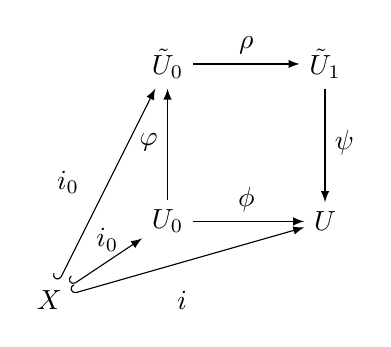
\begin{tikzpicture}

\node (v3) at (-1,1) {$U_0$};
\node (v2) at (1,1) {$U$};
\node (v1) at (-2.5,0) {$X$};

\node [above left] at (-1.5,0.5) {$i_0$};
\node [right] at (-1,0) {$i$};

\draw [-latex] (v3) edge (v2);
\draw[right hook -latex] (v1) edge (v2);
\draw [right hook -latex]  (v1) edge (v3);

\node [above] at (0,1) {$\phi$};

\node (U0') at (-1,3) {$\tilde{U}_0$};
\node (U1') at (1,3) {$\tilde{U}_1$};

\draw [-latex] (U0') edge (U1');

\node [above] at (0,3) {$\rho$};
%\draw [-latex] plot[smooth, tension=.7] coordinates {(-0.25,-0.5) (-2,0.5) (-2,2.5) (-1.25,3)};
\node [left] at (-2,1.5) {$i_0$};

\draw [-latex] (v3) edge (U0');
\node [left] at (-1,2) {$\varphi$};

\draw [-latex] (U1') edge (v2);
\node [right] at (1,2) {$\psi$};

\draw [right hook -latex] (v1) edge (U0');
\end{tikzpicture}.
		\end{center}
\end{proof}

\begin{proof}[Proof of \autoref{thm:Weinstein2}]
	Let us select any Riemannian metric on $M$, with respect to which we can define $W \coloneqq T_pX^\perp$. By definition, we have that $T_pX$ is a Lagrangian subspace of $(T_pM, \omega_0|_p \eqqcolon \Omega_0)$ and $(T_pM, \omega_1|_p \eqqcolon \Omega_1)$. We can then invoke Lemma \autoref{lem:Weinstein2} to obtain a map $H|_p: T_pM \to T_pM$ such that $\left( H|_p \right) |_{T_pX} \equiv \mathrm{Id}_{T_pX}$, and $H|_p^* \Omega_1 = \Omega_0$. As suggested by the notation, the definition of such a map $H|_p$ at each $p \in M$ gives a smooth tensor field. In fact, due to a result by Whitney, we can define a neighbourhood of $X$ in $M$ with an embedding $h: N \hookrightarrow M$ such that $h|_X \equiv \mathrm{Id}_x$ and $H \equiv dh$.
\end{proof} 

\begin{lemma}\label{lem:Weinstein2}
	I can assert whatever I like
\end{lemma}

\section{Almost Complex Structures and K\"ahler Manifolds}

\paragraph{} The three key branches of differential geometry are similar in that they are all specified by particular tensor fields defined over a differentiable manifold:
	\begin{center}
		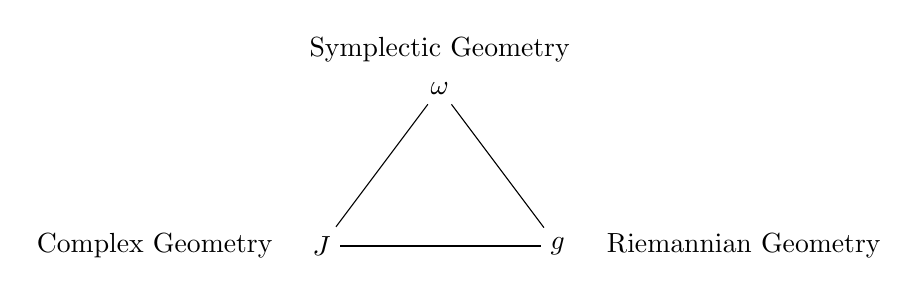
\begin{tikzpicture}

\node (v2) at (0,1) {$\omega$};
\node (v1) at (-1.5,-1) {$J$};
\node (v3) at (1.5,-1) {$g$};
\draw  (v1) edge (v2);
\draw  (v2) edge (v3);
\draw  (v3) edge (v1);

\node at (0,1.5) {Symplectic Geometry};
\node [left] at (-2,-1) {Complex Geometry};
\node[right] at (2,-1) {Riemannian Geometry};

\end{tikzpicture}.
	\end{center}
	The tensors in question are defined on their fibres as
		\begin{align*}
			\omega|_p :T_pM &\times T_pM \to \mathbb{R}, & \mathrm{Skew-symmetric bilinear map},\\
			g|_p: T_pM &\times T_pM \to \mathbb{R}, & \mathrm{Positive definite bilinear map}, \\
			J|_p: T_pM &\to T_pM, & \mathrm{Satisfying } J^2 = -\mathds{1}.
		\end{align*}
		
\begin{definition}[Complex Structure (Vector Space)]
	A \textbf{complex structure} on a vector space $V$ is a linear map
		\begin{align}
			J: V \to V, \text{ such that} \quad J^2 = - \mathds{1}.
		\end{align}	
\end{definition}

\begin{definition}[Compatible (Complex Structure)]\label{def:compatibility}
	Given a symplectic vector space $(V,\Omega)$, a complex structure is \textbf{compatible} if the map $G_J(u,v) \coloneqq \Omega(u,Jv)$ defines an inner product. Explicitly, for all $u,v \in V$, we must have
		\begin{align*}
			\Omega(Ju,Jv) &= \Omega(u,v),  &\Rightarrow& \, G_J \text{ is symmetric},\\
			\Omega(v,Jv) &\geq 0,  &\Rightarrow& \, G_J \text{ is positive definite}.
		\end{align*}
\end{definition}

\begin{prop}[Polar Decomposition]
	Given a symplectic vector space $(V,\Omega)$ with inner product $G$, we can \textit{canonically} construct a compatible complex structure $J$.
\end{prop}
\begin{remark}
	Note that the inner product $G_J$ is not equivalent to $G$ in general.
\end{remark}

\begin{proof}
	We have two non-degenerate bilinear forms on $V$, meaning that, if $\hat{g}: V^* \to V$ is the induced isomorphism such that $\iota_{\hat{g}(W)}G = W$, then we have a linear map ${A(v) = \hat{g}(\iota_v \Omega)}$, i.e. $\iota_v \Omega = \iota_{A(v)} G$. If $A^2 = - \mathrm{Id}$, then $G = G_A$ and we are done, otherwise we can show that $A$ is skew-adjoint with respect to $G$ as, $\forall u,v \in V$
		\begin{align}
			G(Au,v) = \Omega(u,v) = -\Omega(v,u) = - G(Av,u) = G(A^tv,u).
		\end{align}
	Thus $-A^2$ is symmetric and positive definite, as $G(-A^2u,u) = G(A^tu,A^tu) \geq 0$, from these we can establish that $-A^2$ is diagonalisable, i.e. $-A^2 = BDB^{-1}$. Thus we define, $J = B D^{-\tfrac{1}{2}} B^{-1} A$, this implies that $J^2 = $. Assuming that $A$ commutes with $BD^{-\tfrac{1}{2}}B^{-1}$, we then have that $J^2 = -\mathds{1}$, and we can check that $J$ is compatible with $\Omega$. We further have that $G_J(u,v) = G(\sqrt{AA^T}u,v)$, which is distinct from $G$. We call $A = \sqrt{AA^T}J$ the \textbf{polar decomposition} of $A$.
\end{proof}

\begin{prop}
	Let $(V,\Omega)$ be a symplectic vector space, and let $\mathcal{J}$ denote the set of all complex structures on $V$ compatible with $\Omega$, then $\mathcal{J}$ is path connected.
\end{prop}
\begin{proof}
	Let $J_0, J_1 \in \mathcal{J}$. We define a straight line homotopy between their induced inner products, $G_t \coloneqq (1-t) G_{J_0} + t G_{J_1}$. For each $t$, we have a polar decomposition of the associated $A_t = \sqrt{A_t A_t^T}J_t$. The family $\{J_t\}_{t=1}^1$ gives the required path.
\end{proof}

\begin{definition}[Almost Complex Structure]
	An \textbf{almost complex structure} $J$ on a manifold $M$ is a smooth tensor field such that $J|_p$ is a complex structure on $T_pM, \forall p \in M$.
\end{definition}

\begin{definition}[Integrable (Almost Complex Structure)]
	An almost complex structure $J$ on $M$ is \textbf{integrable} if there exists locally a set of coordinates $(x^i,y^i)_{i=1}^n$ of $M$ such that
		\begin{align}
			J \frac{\partial}{\partial x^i} =  \frac{\partial}{\partial y^i}, \quad J \frac{\partial}{\partial y^i} = - \frac{\partial}{\partial x^i}
		\end{align}
\end{definition}

\begin{definition}[Compatible (Almost Complex Structure)]
	An almost complex structure $J$ on a symplectic manifold $(M,\omega)$ is \textbf{compatible} with $\omega$ if $J|_p$ is compatible with $\omega_p, \forall p \in M$. We then call $(\omega, g_J, J)$ a \textbf{complex triple}, where $g_J|_p \equiv G_{J|_p}$. 
\end{definition}
\begin{remark}
	Similarly to before, fixing any two of the complex triple allows us to canonically construct the third.
\end{remark}

\begin{prop}
	Let $\mathfrak{J}$ denote the set of almost complex structures compatible on a symplectic manifold $(M,\omega)$, the $\mathfrak{J}$ is contractible.
\end{prop}
\textbf{Proof Omitted.}

\begin{prop}
	An almost complex structure on $M$ is compatible with two symplectic forms, $\omega_0$ and $\omega_1$, on $M$ if and only iff $\omega_0$, $\omega_1$ are deformation equivalent.
\end{prop}
\textbf{Proof Omitted.}

\begin{theorem}[Gromov]
	Let $(M,J)$ be an almost complex manifold. If $M$ is open (i.e. it contains no closed connected components), then there exists a symplectic form $\omega$ in any given $2$-cohomology class such that $J$ is homotopic to an almost complex structure compatible with $\omega$.
\end{theorem}

\begin{definition}[Almost Complex Submanifold]
	An \textbf{almost complex submanifold} $X$ of an almost complex manifold $(M,J)$ is a submanifold $X \subset M$ such that $\forall p \in X$, $ J|_p  \left(T_pX\right) = T_pX$.
\end{definition}

\begin{prop}\label{prop:almostCplxSymp}
	Let $(M,\omega)$ be a symplectic manifold with compatible almost complex structure $J$. If $X \subset M$ is an almost complex submanifold of $(M,J)$, then $X$ is a symplectic submanifold of $(M,\omega)$, i.e. $(X,i^*\omega)$ is symplectic.
\end{prop}
\begin{proof}
	As pullbacks commute with $d$, $i^* \omega$ is closed. It is also non-degenerate, as $\forall v \in T_pX$
		\begin{equation}
			\omega|_p (v, J|_p v) = G_{J|_p} ( J|_p v, J|_p v) \geq 0
		\end{equation}
\end{proof}

\subsection{Dolbeaut Theory}

\begin{definition}[Complexified Tangent Bundle]
	The \textbf{complexified tangent bundle} of a manifold $M$ is the vector bundle $TM \otimes \mathbb{C} \to M$, i.e. the fibres are $T_pM$ but over the complex field instead.
\end{definition}
\begin{remark}
	Given an almost complex manifold $(M,J)$, we can extend $J$ to the complexified tangent bundle by $J(v \otimes z) = (Jv) \otimes z, \forall z \in \mathbb{C}$. This map can then be said to have eigenvalues $\pm i$.
\end{remark}

\begin{definition}[(Anti-)Holomorphic Tangent Spaces]
	Let $(M,J)$ be an almost complex manifold, and let $TM \otimes \mathbb{C}$ be the complexified tangent bundle of $M$. Then the \textbf{$J$-holomorphic tangent bundle} is defined by
		\begin{equation}
			T_{1,0} \coloneqq\{ v \in TM \otimes \mathbb{C} : Jv = iv\} \equiv \{ v \otimes 1 - (Jv) \otimes i\}_{v \in TM}.
		\end{equation}
	Similarly, we define the \textbf{$J$-antiholomorphic tangent bundle} as
		\begin{equation}
			T_{0,1} \coloneqq\{ v \in TM \otimes \mathbb{C} : Jv = -iv\} \equiv \{ v \otimes 1 + (Jv) \otimes i\}_{v \in TM}.
		\end{equation}
\end{definition}
\begin{remark}
	We can think of $T_{1,0}$ and $T_{0,1}$ as the decomposition of $TM \otimes \mathbb{C}$, as we have the map
		\begin{align*}
			TM \otimes \mathbb{C} &\congto T_{1,0} \oplus T_{0,1},\\
			v & \mapsto \tfrac{1}{2} (v - iJv, v+iJv).
		\end{align*}
	We can also do the same with the cotangent bundle. Using the pullback of $J$, ${(J|_p)^* \xi \coloneqq \xi \circ J|_p}$, we define the decomposition
		\begin{align*}
			T^*M \otimes \mathbb{C} &\congto T^{1,0} \oplus T^{0,1},\\
			\xi & \mapsto \tfrac{1}{2} (\xi - iJ^*\xi, \xi+iJ^*\xi).
		\end{align*}
	Similarly to before, we call elements of each side of the composition \textbf{complex (anti)linear functionals}, as $\xi( u + Jv) = \xi(u) \pm i\xi(v)$ respectively.
\end{remark}

\begin{prop}\label{prop:extDecomp}
	The exterior spaces of the complexified cotangent bundle can be decomposed as
		\begin{equation}
			\Lambda^k\left( T^*M \otimes \mathbb{C} \right) = \bigoplus_{l+m =k} \left[ \left( \Lambda^l T^{1,0} \right) \otimes \left( \Lambda^m T^{0,1} \right) \right] \eqqcolon \Lambda^{l,m}
		\end{equation}
\end{prop}

\begin{definition}[Differential Forms of type $(l,m)$]
	Decomposing $\Omega^k(M;\mathbb{C})$, the complex-valued $k$-forms on $M$ according to \autoref{prop:extDecomp}, we have
		\begin{equation}
			\Omega^k(M;\mathbb{C}) = \bigoplus_{l+m=k} \Gamma\left(\Lambda^{l,m}\right) \eqqcolon \bigoplus \Omega^{l,m}.
		\end{equation}
	Then, elements $\omega \in \Omega^{l,m}$ are called \textbf{differential forms of type $(l,m)$}
\end{definition}
\begin{remark}
	The exterior derivative decomposes accordingly into $\partial$ and $\bar{\partial}$. Let $\pi^{l,m}: \Omega^k(M; \mathbb{C}) \to \Omega^{l,m}$ be the appropriate projection under the above decomposition. Then on $\Omega^k(M;\mathbb{C})$ we have
		\begin{align}
			\partial = \pi^{l+1, m} \circ d, \quad \bar{\partial} = \pi^{l, m+1} \circ d.
		\end{align}
	We can visualise this using the following diagram:
		\begin{center}
			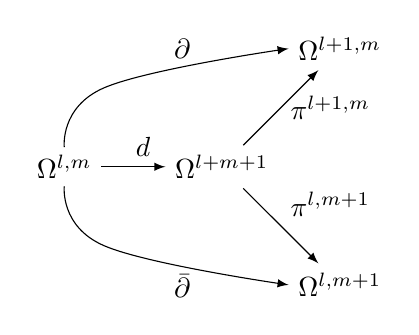
\begin{tikzpicture}

\node (v1) at (-1,0) {$\Omega^{l,m}$};
\node (v2) at (1,0) {$\Omega^{l+m+1}$};
\node (v3) at (2.5,1.5) {$\Omega^{l+1,m}$};
\node (v4) at (2.5,-1.5) {$\Omega^{l,m+1}$};

\draw [-latex] (v1) edge (v2);
\draw [-latex] (v2) edge (v3);
\draw [-latex] (v2) edge (v4);

\node [above] at (-0.,0) {$d$};

\node [right] at (1.75,0.75) {$\pi^{l+1,m}$};
\node [above right] at (1.75,-0.75) {$\pi^{l,m+1}$};

\draw [-latex] plot[smooth, tension=.7] coordinates {(-1,0.25) (-0.5,1) (1.85,1.5)};
\draw [-latex] plot[smooth, tension=.7] coordinates {(-1,-0.25) (-0.5,-1) (1.85,-1.5)};

\node [below] at (0.5,-1.25) {$\bar{\partial}$};
\node [above] at (0.5,1.25) {${\partial}$};

\end{tikzpicture}
		\end{center}
	It is important to note, however, that if $k>0$, \textit{this decomposition is not complete}. For a differential form $\beta$ of type $(l,m)$, where $l+m=k$ the full decomposition is
		\begin{equation}
			d\beta = \pi^{k+1,0}(d\beta) + \pi^{k,1}(d\beta) + \cdots + \partial \beta + \bar{\partial} \beta + \cdots + \pi^{0,k+1}(d\beta).
		\end{equation}
\end{remark}

\begin{definition}[$J$-Holomorphic]
	A complex valued function $f \in C^\infty(M;\mathbb{C})$ is $J$\textbf{-holomorphic} if $\bar{\partial}f = 0$, and $J$\textbf{-antiholomorphic} if $\partial f =0$.
\end{definition}
\begin{remark}
	Note that these definitions can be shown to be equivalent to the conditions $df|_p \in T_p^{1,0}$ and $df|_p \in T_p^{0,1}$ respectively.
\end{remark}

\begin{theorem}[Newlander-Nirenberg]\label{thm:N-N}
	Let $(M,J)$ be an almost complex manifold. Then the following are equivalent
		\begin{enumerate}[label = (\roman*), itemsep=0pt, align = center]
			\item \label{itm:NN1} $\bar{\partial}^2 = 0$,
			\item \label{itm:NN2} $\partial^2 = 0$,
			\item \label{itm:NN3} $d = \partial + \bar{\partial}$,
			\item \label{itm:NN4} $J$ is integrable,
			\item \label{itm:NN5} $N(X,Y) \coloneqq [JX,JY] - J[JX,Y] - J[X,JY] - [X,Y] \equiv 0$.\footnote{The operator $N$ is known as the \textbf{Nijenhuis tensor}.}
		\end{enumerate}
\end{theorem}
\begin{remark}
	From \autoref{itm:NN1} and \autoref{itm:NN2} we have that $\bar{\partial}$ and $\partial$ each form a cochain complex on $\Omega^{l,m+n}$ and $\Omega^{l+n,m}$ respectively.
	Next, \autoref{itm:NN4} implies that $T_{1,0}$ and $T_{0,1}$ are both integrable distributions over $M$. We can also define a set of coordinates $(z^i,\bar{z}^i)$ such that
		\begin{align}\label{eq:JCanon}
			J \frac{\partial}{\partial z^i} = i \frac{\partial}{\partial z^i}, \quad J \frac{\partial}{\partial \bar{z}^i} = -i \frac{\partial}{\partial \bar{z}^i}.
		\end{align}
	In other words, without complexifying $M$ itself, we can loosely say that $z^i = x^i + i y^i$, and $\bar{z}^i = x^i - i y^i$. We then call $J$ the \textbf{canonical almost complex structure} on $M$.
\end{remark}

\begin{definition}[Dolbeault Cohomology]
	For an almost complex manifold $(M,J)$ where $J$ is integrable, we define the \textbf{Dolbeault cohomology} using the cochain complex of $\bar{\partial}$
		\begin{equation}
			H^{l,m}_{\mathrm{Dolbeault}}(M) \coloneqq \frac{
				\mathrm{Ker} \Big( \bar{\partial}: \Omega^{l,m} \to \Omega^{l,m+1} \Big)
			}{
				\mathrm{Im} \Big( \bar{\partial}: \Omega^{l,m-1} \to \Omega^{l,m} \Big)
			}.
		\end{equation}
\end{definition}
\begin{remark}
	Given a canonical chart $(z^i,\bar{z}^i)$ for an almost complex manifold $(M,J)$, we can locally express a differential form $\beta$ of type $(l,m)$ as
		\begin{equation}
			\beta = \sum_{|I| = l, |J| = m} B_{I,J} dz^I \wedge d\bar{z}^J.
		\end{equation}
	Where we are using multi-index notation $I = \{ i_1 < \ldots < i_{|I|} \}$, $dz^I = dz^{i_1} \wedge \cdots \wedge dz^{i_{|I|}}$.
	The exterior derivative in these coordinates is given by
		\begin{align}
			d\beta = \sum_{l+m=k} \sum_{I,J} \left( 
			\underbrace{
					 \partial \beta_{I,J} \wedge dz^I \wedge d\bar{z}^J
			}_{\in \Omega^{m+1,l}} + \underbrace{
				\bar{\partial} \beta_{I,J} \wedge dz^I \wedge d\bar{z}^J
			}_{\in \Omega^{m,l+1}} \right).
		\end{align}
	From this we can conclude that the existence of a chart satisfying \eqref{eq:JCanon} implies \ref{itm:NN1} to \ref{itm:NN4} of \autoref{thm:N-N} hold.
\end{remark}

\subsection{K\"ahler Manifolds}

\begin{definition}[K\"ahler Manifold]
	A \textbf{K\"ahler manifold} is a triple $(M,\omega,J)$ such that $\omega$ is a symplectic form on $M$ and $J$ is both integrable and compatible with $\omega$. We then refer to $\omega$ as a \textbf{K\"ahler form}
\end{definition}

\begin{prop}
	Let $(M,\omega,J)$ be a K\"ahler manifold, then
	\begin{ronumerate}
		\item $\omega \in \Omega^{1,1}$,
		\item $\omega$ is $\partial$ and $\bar{\partial}$ closed (and thus defines a Dolbeault cohomology class).
	\end{ronumerate}

\end{prop}
\begin{proof}
	Na\"ively, we can write the decomposition $\omega = \omega^{2,0} + \omega^{1,1} + \omega^{0,2}$, where ${\omega^{l,m} \in \Omega^{l,m}}$. Recall that from \autoref{def:compatibility}, we must have that $J^*\omega = \omega, \Rightarrow J^* \omega^{l,m} = \omega^{l,m}$. In general, the action of $J$ on the above decomposition is
		\begin{equation}
			J^* \omega = (i \cdot i) \omega^{2,0} + (i \cdot (-i)) \omega^{1,1} + ((-i) \cdot (-i)) \omega^{0,2}.\footnote{The general result is that, for $\eta \in \Omega^{l,m}, J^*\eta = i^{l-m} \eta$.}
		\end{equation}
	Thus $\omega = \omega^{1,1}$. Next, as $\omega$ is closed, and from \autoref{thm:N-N} we have that $d = \partial + \bar{\partial}$
		\begin{equation}
			d\omega = 0 = \underbrace{\partial \omega}_{\in \Omega^{2,1}} + \underbrace{\bar{\partial} \omega}_{\in \Omega^{1,2}}.
		\end{equation}
	As these belong to different parts of the decomposition of $\Omega^2$, they must both vanish.
\end{proof}
\begin{remark}
	Using a set of `complex' coordinates $(z^i,\bar{z}^i)$ we can express $\omega$ locally as
		\begin{equation}
			\omega = \tfrac{i}{2} \sum_{i,j = 1}^n h_ij dz^i \wedge d\bar{z}^j,
		\end{equation}
	in which case the matrices $\big(h_ij(p)\big)$ must be Hermitian and positive definite.
\end{remark}

\begin{definition}[Strictly Plurisubharmonic]
	Let $M$ be a complex manifold with a \textit{real} valued function $\rho$. This function is \textbf{strictly plurisubharmonic} if locally the matrices $\left(\frac{\partial^2 \rho}{\partial z^i \partial \bar{z}^j} \right)$ are positive definite.
\end{definition}

\begin{prop}
	Let $M$ be a complex manifold with strictly plurisubharmonic function $\rho$. Then $\omega = \tfrac{i}{2} \partial \bar{\partial} \rho$ is a K\"ahler form. Such a function $\rho$ is known as a \textbf{K\"ahler potential}.
\end{prop}
\begin{proof}
	Immediately we have that $\omega \in \Omega^{1,1}$ and $\partial \omega = 0$. Using the fact that $\partial$ and $\bar{\partial}$ anti-commute, we can readily verify that $\omega$ is also $\bar{\partial}$ closed. The final conditions needed for $\omega$ come from the fact that $h_ij = \left(\frac{\partial^2 \rho}{\partial z^i \partial \bar{z}^j} \right)$.
\end{proof}

\begin{prop}
	Let $M$ be a complex manifold with a real valued differential form $\omega$ of type $(1,1)$. Then $\forall p \in M$, there exists a neighbourhood $U \ni p$ and function $\rho \in C^\infty(U; \mathbb{R})$ such that $\omega|_U \equiv \tfrac{i}{2}\partial\bar{\partial} \rho$.
\end{prop}
\begin{proof}
	\textit{Basically just apply holomorphic version of the Poincar\'e lemma:}
		\begin{equation}
			\forall p \in M, \; \exists \text{ a neighbourhood } U \ni p, \text{ such that } H^{l,m}_{\mathrm{Dolbeault}}(U) = 0, \forall m > 0.
		\end{equation}
\end{proof}
\begin{remark}
	It is \textit{impossible} to have a global K\"ahler potential on a closed, compact K\"ahler manifold. This is because $\omega$ would then be exact, which would mean the volume form $\omega^n$ on $M$ would be ill defined.
\end{remark}

\begin{example}
	\begin{ronumerate}
		\item Let $M = \mathbb{C}^n$, $\rho(z) = \ln(|z|^2+1)$, then $ \omega_{\mathrm{FS}} \coloneqq \tfrac{i}{2} \partial \bar{\partial} (\ln(|z|^2+1))$ is known as the \textbf{Fubini-Study Form} on $\mathbb{C}^n$.
		\item Let, $M = \mathbb{CP}^n$ and define the standard charts $(U_j, \phi_j)$ such that 
			\begin{align*}
				U_j &\coloneqq \{ [z] \in \mathbb{CP}^n | z_j \neq 0 \},\\
				\phi_j([z]) &= \left( \tfrac{z_0}{z_j}, \cdots \tfrac{z_{j-1}}{z_j},\tfrac{z_{j+1}}{z_j}, \cdots \tfrac{z_n}{z_j}\right).
			\end{align*}
		We can then extend the definition of the Fubini-Study form to $M$ by `gluing together' the forms $\phi_j^*\omega_\mathrm{FS}$. This is well defined as 
		\begin{equation}
			\left(\phi_i^*\omega_\mathrm{FS}\right)|_{U_i \cup U_j} \equiv \left(\phi_j^*\omega_\mathrm{FS}\right)|_{U_i \cup U_j}
		\end{equation}
	\end{ronumerate}
\end{example}

\begin{prop}
	Let $(M,\omega,J)$ be a K\"ahler manifold such that $M$ is complex, and $J$ is its canonical almost complex structure. Let $X$ be a complex submanifold with inclusion map $i: X \hookrightarrow M$, then $(X,i^*\omega, i^*J)$ is a K\"ahler submanifold.
\end{prop}
\begin{proof}
	As $X$ is an almost complex submanifold \autoref{prop:almostCplxSymp} tells us that $(X,i^*\omega)$ is symplectic. Thus we just need to convince ourselves of the compatibility of $i^*J$ and $i^*\omega$. 
\end{proof}
\begin{remark}
	Similarly, restricting a K\"ahler \textit{potential} to a submanifold $X \subset M$ defines a K\"ahler potential on $X$, as the Hessian of a restriction is a principle minor of the overall Hessian and thus inherits the positive definite property.
\end{remark}

\begin{example}[Examples of K\"ahler Manifolds]
	\begin{ronumerate}
		\item Complex submanifolds of $\left( \mathbb{C}^n,\omega_0 \right)$
		\item Complex submanifolds of $\left( \mathbb{C}^n,\omega_\mathrm{FS} \right)$
		\item Complex submanifolds of $\left( \mathbb{CP}^n,\omega_\mathrm{FS} \right)$
		\item Riemann Surfaces
		\item Products of K\"ahler manifolds
	\end{ronumerate}
\end{example}

\subsection{Hodge Theory}

\begin{theorem}[Hodge]
	Let $(M,\omega,J)$ be a compact K\"ahler manifold, then
		\begin{equation}
			H^k_\mathrm{dR}(M;\mathbb{C}) \simeq \bigoplus_{l+m=k} H^{l,m}_\mathrm{Dol}(M).
		\end{equation}
\end{theorem}

\subsubsection{Hodge theory for real manifolds}

\begin{definition}[Inner Product Extension]
	Let $V$ be a real, $m$-dimensional, oriented\footnote{I.e. there is specified, up to multiplication by a positive scalar, a top from $\epsilon \in \Lambda^n V$.} vector space. Given an inner product $G: V \times V \to \mathbb{R}$, we can define the \textbf{extension} of $G$ to $\Lambda^k(V)$ by
		\begin{equation}
			\langle u_1 \wedge \cdots \wedge u_k, v_1 \wedge \cdots \wedge v_k \rangle = \mathrm{Det}\left(G(u_i,v_j)\right).
		\end{equation}
	Alternatively, given an oriented orthonormal basis $\{e_i\}_{i=1}^m$ of $V$, we can define the extension of $G$ by imposing that $\{e_I\}_{|I| = k}$ is an \textit{orthonormal} basis of $\Lambda^k(V)$.
\end{definition}

\begin{definition}[Hodge $\star$ Operator]
	Given a real, $m$-dimensional, oriented vector space $V$ with inner product $G$, the Hodge star operator is a linear map $\star: \Lambda^k(V) \to \Lambda^{m-k}(V)$ such that, for $\alpha, \beta \in \Lambda^k (V)$
		\begin{align}
			\alpha \wedge ( \star \beta ) = \langle \alpha, \beta \rangle e_1 \wedge \cdots \wedge e_m.
		\end{align}
\end{definition}
\begin{remark}
	It is helpful to consider the action of $\star$ on the orthonormal basis:
			\begin{subequations}\begin{align}
				\star( e_1 \wedge \cdots e_k ) &= e_{k+1} \wedge \cdots \wedge e_m, \\
				\star( e_{k+1} \wedge \cdots \wedge e_m ) &= (-1)^{k(m-k)} e_1 \wedge \cdots e_k, \\
				\star( e_1 \wedge \cdots \wedge e_m ) &= 1, \\
				  e_1 \wedge \cdots \wedge e_m &=\star 1 \Rightarrow \star \star = (-1)^{k(m-k)} \mathds{1}.
			\end{align}\end{subequations}
		Also, note that this operator can be defined on real, oriented, Riemannian manifolds without any issue, simply give it the above definition on each tangent space.
\end{remark}

\begin{definition}
	The \textbf{codifferential operator} is a linear map $\delta: \Omega^k \to \Omega^{k-1}$ defined by
		\begin{equation}
			\delta = (-1)^{m(k+1)+1} \star \circ \, d \circ \star.
		\end{equation}
\end{definition}
\begin{remark}
	As $\star^2 \propto \mathds{1}$, we have $\delta^2 = 0$. More interestingly, it can be regarded as the `adjoint' of $d$ as, for $\alpha \in \Omega^k$, $\beta \in \Omega^{k+1}$, we have
		\begin{equation}
			\langle d\alpha, \beta \rangle_{\mathcal{L}^2} \coloneqq \int_M \langle d\alpha, \beta \rangle \mathrm{Vol} = \int_M \langle \alpha, \delta \beta \rangle \mathrm{Vol}.
		\end{equation}
	We also have a neat expression for the volume form, as $\mathrm{Vol} = \star 1$.
\end{remark}\todo{Check}
	
\begin{definition}[Laplace-Beltrami Operator]
	The \textbf{Laplace-Beltrami operator} is a derivation $\Delta: \Omega^k \to \Omega^k$ defined by
		\begin{equation}
			\Delta = d \delta + \delta d.
		\end{equation}
\end{definition}
\begin{remark}\hfill
	\begin{ronumerate}
		\item $\Delta \star = \star \Delta$,
		\item $\Delta = (d + \delta)^2$
		\item $\langle \Delta \alpha, \beta \rangle_{\mathcal{L}^2} = \langle \alpha , \Delta\beta \rangle_{\mathcal{L}^2}$
		\item $\Delta \alpha = 0$ iff $d\alpha = \delta \alpha = 0$.
	\end{ronumerate}
\end{remark}

\begin{definition}[Harmonic ($k$-form)]
	A $k$-form $\alpha$ on an orientable, Riemannian manifold $M$ is \textbf{harmonic} if $\Delta \alpha = 0$. We denote the set of all harmonic $k$-forms on $M$ by $\mathcal{H}^k(M)$.
\end{definition}

\begin{theorem}[Hodge]\label{thm:cplxHodge}
	Let $(M,g)$ be a compact oriented Riemannian manifold, then every cohomology class in $H^k_\mathrm{dR}(M)$ has a unique harmonic representative, i.e.
		\begin{equation}
			H^k_\mathrm{dR}(M) \simeq \mathcal{H}^k.
		\end{equation}
\end{theorem}

\subsubsection{Hodge theory for K\"ahler manifolds}

\begin{prop}
	Let $(M, \omega, J)$ be a $2n$-dimensional K\"ahler manifold, with $\star, d$ and $\delta$ defined using $g_J$. Then these operators satisfy the following
		\begin{ronumerate}
			\item $\star: \Omega^{l,m} \to \Omega^{n-l,n-m}$,
			\item $\Delta: \Omega^{l,m} \to \Omega^{l,m}$,
			\item $\bar{\partial}^* \coloneqq - \star \bar{\partial} \star$ is $\mathcal{L}^2$-adjoint to $\bar{\partial}$, and ${\partial}^* \coloneqq - \star {\partial} \star$ is $\mathcal{L}^2$-adjoint to ${\partial}$,
			\item $\Delta_\partial \coloneqq \partial \partial^* + \partial^* \partial$, $\Delta_{\bar{\partial}} \coloneqq \bar{\partial }\bar{\partial}^* + \bar{\partial}^* \bar{\partial}$, $\Rightarrow \Delta = 2\Delta_\partial = 2 \Delta_{\bar{\partial}}$
		\end{ronumerate}
\end{prop}

\begin{theorem}[Hodge, Complex]
	Let $(M,\omega,J)$ be K\"ahler, then every cohomology class in $H^{l,m}_\mathrm{Dol}(M)$ has a unique harmonic representative in $\mathcal{H}^{l,m}$, where $\mathcal{H}^{l,m} = \pi^{l,m}\left( \mathcal{H}^k \right)$.
\end{theorem}

\subsubsection{Topological Consequences}

\begin{definition}[Betti/Hodge Numbers]
	The \textbf{Betti numbers} and \textbf{Hodge numbers} are defined by
		\begin{align}
			b_k &\coloneqq \mathrm{Dim}_\mathbb{R}\left( H^k_{\mathrm{dR}} (M) \right), \\
			h_{l,m} &\coloneqq \mathrm{Dim}_\mathbb{C} \left( H^{l,m}_\mathrm{Dol}(M) \right)
		\end{align}
\end{definition}
\begin{remark}\hfill
	\begin{itemize}
		\item The complex Hodge theorem \ref{thm:cplxHodge} implies that $b_k = \sum_{l+m=k} h_{l,m}$.
		\item $H^{l,m}_{\mathrm{Dol}} \simeq H^{m,l}_{\mathrm{Dol}} \Rightarrow h_{l,m} = h_{m,l}$ \hfill {\textbf{Hodge Symmetry}}
		\item $H^{l,m}_{\mathrm{Dol}} \simeq H^{n-l,n-m}_{\mathrm{Dol}} \Rightarrow h_{l,m} = h_{n-l,n-m}$ \hfill \textbf{Central Symmetry/Serre Duality}
		\item Odd Betti numbers are even, as $b_{2k+1} = \sum_{l+m = 2k+1}h_{l,m} = 2\left(\sum_{l=0}^k h_{l,2k-l} \right)$
		\item Even Betti numbers are positive
		\item $h_{1,0} = h_{0,1} = \tfrac{1}{2}b_1$ is a topological invariant
		\item $h_{k,k}$ is positive, as $\omega^k \in \Omega^{k,k}$ is closed but not exact
	\end{itemize}
\end{remark}

\section{Classical Mechanics}

\subsection{Hamiltonian Vector Fields}

\begin{definition}[Hamiltonian Function/Vector Field]
	Given a function $H$ on a symplectic manifold $(M,\omega)$ let $X_H$ be the unique vector field such that
		\begin{equation}
			dH = \iota_{X_H} \omega.
		\end{equation}
	Then $X_H$ is a \textbf{Hamiltonian vector field} with \textbf{Hamiltonian function} $H$.
\end{definition}

\begin{prop}
	Given a Hamiltonian vector field $X_H$ which is \textit{complete}, we can integrate it to obtain a flow $\rho_t$. Then, $\rho_t$ is a family of \textit{symplectomorphisms}, preserving $\omega$. The flow also preserves $H$, i.e. $\rho_t^* H \equiv H$.
\end{prop}
\begin{proof}
	\begin{equation}
		\frac{d}{dt} \rho^*_t \omega = \rho^*_t(\mathcal{L}_{X_H} \omega) = \rho^*_t \left( d \circ \underbrace{\iota_{X_H} \omega}_{=d\omega} + \iota_{X_H} \underbrace{\circ d \omega}_{=0} \right) = 0.
	\end{equation}
	Thus $\rho^*_t \omega = \rho^*_{t'} \omega$ is independent of $t$. Noting that $\rho_0 = \mathrm{Id}$ is trivially a symplectomorphism, the result then holds for all $t$.
	
	Next, note that $X_H H = \mathcal{L}_{X_H} H = \iota_{X_H} dH = \iota_{X_H} ( \iota_{X_H} \omega ) = 0$, where the last term vanishes as $\omega$ is skew. Finally, note that $\nicefrac{d}{dt} (\rho^*_t H) = X_H H = 0$, and similarly to before $\rho_0 = \mathrm{Id}$ gives the desired result.
\end{proof}

\begin{definition}[Symplectic Vector Field]
	Let $(M,\omega)$ be a symplectic manifold. A vector field $X \in \mathfrak{X}(M)$ is \textbf{symplectic} if $\mathcal{L}_X \omega = 0$, i.e. locally, the flows of $X$ are symplectomorphisms.
\end{definition}

\begin{remark}
	Hamiltonian and symplectic vector fields are comparable to exact and closed differential forms respectively. We could alternatively define $X$ as Hamiltonian if $\iota_X \omega$ is exact, and symplectic if $\iota_X \omega$ is closed, the latter owing to the fact that $\mathcal{L}_X \omega = d (\iota_X \omega)$. Hence all Hamiltonian vector fields are symplectic, and locally all symplectic fields are Hamiltonian. Globally, the difference between Hamiltonian and symplectic vector fields $X$ and $Y$ satisfies $\iota_{(X-Y)} \omega \in H^1_{\mathrm{dR}}(M)$.
\end{remark}

\begin{prop}\label{prop:HamiltonianLieBracket}
	Let $X$ and $Y$ be two symplectic vector fields on a symplectic manifold $(M,\omega)$, then their Lie bracket $[X,Y]$ is Hamiltonian.
\end{prop}
\begin{proof}
	One can show that, for any differential form\todo{Prove} $\alpha$, $\iota_{[X,Y]} \alpha \equiv [\iota_X, \mathcal{L}_y] \alpha$. Thus, we have
		\begin{align}
			\iota_{[x,y]} \omega &= \iota_X \circ \cancel{\mathcal{L}_Y \omega} - \mathcal{L}_Y \circ \iota_X \omega, \nonumber \\
			&= - d \circ \iota_Y \circ \iota_X \omega - \iota_y \circ \cancel{ d (\iota_X \omega) }, \nonumber \\
			&= d \left( \omega(Y,X) \right).
		\end{align}
	Thus $[X,Y]$ is Hamiltonian, with Hamiltonian function $\omega([Y,X])$.
\end{proof}

\begin{definition}[Poisson Bracket]
	Given two functions $f,g$ on a symplectic manifold $(M,\omega)$, the Poisson bracket is a bilinear map $\{ \cdot, \cdot \} : C^\infty(M) \times C^\infty(M) \to C^\infty(M)$ defined by
		\begin{equation}
			\{ f,g \} = \omega(X_f,X_g).
		\end{equation}
\end{definition}

\begin{remark}\hfill
	\begin{itemize}
		\item The skew-symmetry of $\omega$ implies that the Poisson bracket is also skew-symmetric. The closedness of $\omega$ implies that the Poisson bracket satisfies the \textit{Jacobi identity}.
		\item Using \autoref{prop:HamiltonianLieBracket}, we can deduce that $[X_f,X_g] = -X_{\{f,g\}}$, thus there exists a natural \textit{Lie algebra anti-isomorphism} between the Poisson bracket on $C^\infty(M)$ and the Lie bracket on the space of Hamiltonian vector fields.
		\item Note that $\omega(X_f,X_g) = \left(\iota_{X_f} \omega \right) X_g = df(X_g) = X_g \circ f$. Thus one can easily show that the Poisson bracket satisfies the Leibniz rule for both of its arguments $\{ f , gh \} = g\{f,h\} + \{f,g\}h$.
		\item From this we also have that $\{f,g\} = 0$ iff $f$ is constant along flows of $X_g$ and vice-versa.
		\item Given a set of Darboux coordinates $(q^i,p_i)$, we can locally express the Hamiltonian vector field of $f$ as
			\begin{equation}
				X_f = \sum_{i=1}^n \left( \frac{\partial f}{\partial p_i} \frac{\partial }{\partial q ^i} - \frac{\partial f}{\partial q ^i} \frac{\partial }{\partial p_i} \right),
			\end{equation}
		and the Poisson bracket as
			\begin{equation}
				\{f,g\} = \sum_{i=1}^n \left( \frac{\partial f}{\partial q^i} \frac{\partial g}{\partial p_i} - \frac{\partial f}{\partial p_i} \frac{\partial g}{\partial q ^i} \right).
			\end{equation}
	\end{itemize}
\end{remark}\todo{Proof of Jacobi}

\subsection{Integrable Systems}

\begin{definition}[Hamiltonian System]
	A \textbf{Hamiltonian system} is a triple $(M,\omega,H)$, where $(M,\omega)$ is a symplectic manifold, and $H \in C^\infty(M)$.
\end{definition}

\begin{definition}[Integral of Motion]
	An \textbf{integral of motion}/\textbf{constant of motion}/\textbf{first integral} for a Hamiltonian system $(M,\omega,H)$ is a function $f$ such that $\{f,H\} = 0$.
\end{definition}
\begin{remark}
	Trivially $H$ itself is a first integral, as are any constant multiples of it. Clearly we also need a notion to distinguish between `different' first integrals
\end{remark}

\begin{definition}[Independent (Functions on a Manifold)]
	A set of functions $\{f_i\}_{i=1}^N$ on a manifold $M$ are \textbf{independent} if, $\forall p \in \tilde{M}$, a dense subset of $M$, the maps $\{df_i|_p\}_{i=1}^N$ are all linearly independent.
\end{definition}

\begin{definition}[Commuting (Functions on a Manifold)]
	A set of functions $\{f_i\}_{i=1}^N$ on a symplectic manifold $(M,\omega)$ \textbf{commute} if $\{f_i,f_j\} = 0, \forall i,j \in \{1,\cdots, N\}$.
\end{definition}

\begin{remark}
	Let $\{f_i\}_{i=1}^N$ be a set of independent commuting functions on a symplectic manifold $(M,\omega)$. Then $\{X_{f_i}|_p\}_{i=1}^N$ span an isotropic subspace of $T_pM$. The fact that the $df_i|_p$ are linearly independent means that the $X_{f_i}|_p$ are too. Thus $N$ is the dimension of the isotropic subspace, which means $\mathrm{Dim}(M) \geq 2N$.
\end{remark}

\begin{definition}[Completely Integrable]
	A Hamiltonian system is \textbf{completely integrable} if it has $n = \tfrac{1}{2}\mathrm{Dim}(M)$ independent, commuting first integrals.
\end{definition}

\begin{example}[Simple/Spherical Pendulum]
	\begin{itemize}
		\item {[Simple Pendulum]} Let $M = T^*S^1$, and let $H(\theta,p) = \tfrac{p^2}{2m} + mg\cos(\theta)$ be the total energy. As $n=1$, $H$ is the only function we need (though the independence condition requires $dH$ to not vanish on a dense subset of $M$.
		\item {[Spherical Pendulum]} Let, $M = T^*S^2$ have the chart $(\phi,\theta, \eta, \xi)$ . Its Hamiltonian is then
			\begin{equation}
				H(\phi, \theta, \eta, \xi) = \frac{1}{2m}\left( \eta^2 + \frac{\xi^2}{\sin^2 \theta} \right) + mg\cos(\theta)
			\end{equation}
	\end{itemize}
\end{example}\todo{Complete}

\begin{remark}
	Note that for a completely integrable system with $f_1 = H$, each of the first integrals is preserved under the flow of $H$, thus orbits under this flow are contained within level sets of $f \coloneqq (f_1,\cdots, f_n)$. If we choose some regular value $c \in \mathbb{R}^n$ of $f$, then the level set $f^{-1}(c)=X$ is an $n$-dimensional submanifold of $M$. Furthermore, as, by definition, $T_pX = \mathrm{Ker}(df|_p) = \mathrm{Span}\{X_{f_1}|_p, \cdots, X_{f_n}|_p\}$, $T_pX$ is an \textit{isotopic} subpace of $(T_pM,\omega|_p)$. Hence, $f^{-1}(c)$ is a Lagrangian submanifold of $(M,\omega)$
\end{remark}

\begin{definition}
	Let $(M,\omega,H)$ be a completely integrable Hamiltonian system with first integrals $\{f_1=H, f_2, \cdots, f_n\}$ and a regular value $c$ of $(f_i)_{i=1}^n$. Then, we can locally define \textbf{angle coordinates} on $f^{-1}(c)$, centred on $p$, as the tuple $(\phi_i)_{i=1}^n$ such that $\phi_i$ is the flow parameter for $X_{f_i}$.
\end{definition}
\begin{remark}
	This is well defined as the flows of $\{X_{f_i}\}$ commute, and locally span $f^{-1}(c)$. If the $X_{f_i}$ are \textit{complete}, then these flows extend to all of $f^{-1}(c)$ connected to $p$. In this case there will be $k$ flows which are periodic, thus the angle coordinate chart induces a diffeomorphism between the connected component of $f^{-1}(c)$ and $\mathbb{R}^{n-k}\times\mathbb{T}^k$.
\end{remark}

\begin{definition}[Liouville Torus]
	Let $(M,\omega,H)$ be a completely integrable Hamiltonian system with first integrals $\{f_1=H, f_2, \cdots, f_n\}$ and a regular value $c$ of $(f_i)_{i=1}^n$. A compact connected component of $f^{-1}(c)$, i.e. one for which $k=n$ in the above remark, is known as a \textbf{Liouville torus}.
\end{definition}

\begin{theorem}[Arnold-Liouville]
	Let $(M\omega,H)$ be an integrable system with first integrals $\{f_1=H, f_2, \cdots, f_n\}$ and a regular value $c$ of $(f_i)_{i=1}^n$. Then
		\begin{ronumerate}
			\item If the flows of $\{ X_{f_i} \}$ are complete, then the connected components of $f^{-1}(c)$ are homogeneous spaces for $\mathbb{R}^n$, i.e. are diffomorphic to $\mathbb{R}^{n-k}\times\mathbb{T}^k$, and admit affine angle coordinates $(\phi_i)_{i=1}^n$
			
			\item There also exists a set of \textbf{action coordinates} $(\psi_i)_{i=1}^n$ such that each $\psi_i$ is an integral of motion and $(\phi_i,\psi_i)_{i=1}^n$ is a Darboux chart.
		\end{ronumerate}
\end{theorem}

\subsection{Variational Principles}

\begin{example}[Classical System of $n$ Particles]
	Given a system of $n$ particles with potential function $V$, we can describe the state of the system in one of two ways
		\begin{ronumerate}
			\item {[Hamiltonian]}\label{itm:Hamiltonian} Using the phase space of the system $T^*\mathbb{R}^{3n}$, the Hamiltonian function $H = \tfrac{1}{2m}\sum_k |p_k|^2 + V(x)$ gives rise to a Hamiltonian vector field, the flow of which corresponds to the time evolution of the system.
			\item \label{itm:Lagrangian }{[Lagrangian]} If we fix two points $x,y \in \mathbb{R}^{3n}$, then the path $\gamma: [0,1] \hookrightarrow \mathbb{R}^{3n}$ taken between them is the one minimising the \textbf{action}
				\begin{equation}
					S[\gamma] = \int_0^1 \left\{ \sum_{k=1}^n \frac{m_k}{2} || \dot{\gamma}_k ||^2 - \gamma^* V \right\} \mathrm{d}t.
				\end{equation}
		\end{ronumerate}
\end{example}
\begin{remark}
	We sometime refer to $\tilde{\gamma}(t) \coloneqq (\gamma(t),\dot{\gamma}(t))$ as the \textbf{lift} of $\gamma$ from $X$ to $T^*X$. We can then define the action corresponding to any Lagrangian function $\mathcal{L}$ as
		\begin{equation}
			S_\gamma \coloneqq \int_0^1 \tilde{\gamma}^* \mathcal{L} \, \mathrm{d}t.
		\end{equation}
	Using a chart $(q_k,v_k)$ on $TM$ compatible with $M$, an extremising condition for the action, the \textbf{Euler-Lagrange equations} can be written
		\begin{equation}
			\frac{\partial \mathcal{L}}{\partial q_k} - \frac{d}{dt}\frac{\partial \mathcal{L}}{\partial v_k} = 0.
		\end{equation}
\end{remark}

\begin{prop}
	The Euler-Lagrange equations are a system second order ODEs if the \textbf{Legendre condition},
		\begin{equation}
			\mathrm{Det}\left(\frac{\partial \mathcal{L}}{\partial v_i \partial v_j} \right) \neq 0,
		\end{equation}
	is met. Furthermore, if the above matrix is positive definite, we say the Lagrangian is \textbf{strictly convex}, and then extremal paths \textit{minimise} the action $S$.
\end{prop}
\begin{definition}[Legendre Transform]
	Given a Lagrangian function $\mathcal{L}: TX \to \mathbb{R}$, the Legendre transformation is a pair of maps $\mathscr{L}: TX \to T^*X$, and $\mathcal{H}: T^*M \to \mathbb{R}$, such that $\mathcal{H} \circ \mathscr{L} = \mathcal{L}$.
\end{definition}
\begin{remark}
	If $\mathcal{L}$ is strictly convex, then the map $\mathscr{L}$ is invertible
\end{remark}
\begin{prop}
	A curve $\gamma$ minimises the action given by the Lagrangian $\mathcal{L}$ iff $\mathscr{L}\circ \tilde{\gamma}$ is an integral curve of the Hamiltonian vector field $X_{\mathcal{H}}$
\end{prop}
\todo[inline]{Improve discussion of Legendre transform}

\section{Hamiltonian Actions}

\begin{definition}[Group Action on a Manifold]
	Let $M$ be a manifold, and let $G$ be a Lie group. An \textbf{action} of the group $G$ on $M$ is a group homomorphism
		\begin{align*}
			\psi:	 G &\to \mathrm{Diff}(M), \\ 
					 g &\mapsto \psi_g, \\
					 \psi_g \circ \psi_h &= \psi_{gh}.
		\end{align*}
\end{definition}

\begin{definition}[Smooth/Symplectic Actions]
	For an action of a group on a manifold, we can define the \textbf{evaluation map}
		\begin{align*}
			e_\psi : M \times G &\to M,\\
					(p,g)	&\mapsto \psi_g(p).
		\end{align*}
	If this is a smooth map, then we say we have a \textbf{smooth action}. If $M$ has a symplectic form $\omega$, then $\psi$ is a \textbf{symplectic action} if $\forall g \in G$, $\psi_g$ is a symplectomorphism.
\end{definition}

\begin{example}
	Group actions of $(\mathbb{R},+)$ are generated as the flows of complete vector fields. These are always smooth and, if $X$ is a symplectic vector field, then its flow is a symplectic action.
\end{example}

\begin{definition}[Hamiltonian Action (of $\mathbb{R}$/$S^1$)]
	An action of $\mathbb{R}$ or $S^1$ is \textbf{Hamiltonian} if it is the flow of a Hamiltonian vector field.
\end{definition}

\begin{remark}
	We should improve this definition. We can relatively easily extend it for an $n$-torus $\mathbb{T}^n$ by requiring that the restriction of $\psi$ to each factor of $\mathbb{T}^n$ satisfies the above condition, \textit{and} if the Hamiltonian function corresponding to each factor is preserved by the action of each other factor. We shall now proceed to build up the formalism in order to extend this definition to the smooth action of \textit{any} Lie group
\end{remark}

\subsection{Lie Theory}

\begin{definition}[Conjugation]
	Given a Lie group $G$, we can define a smooth action of $G$ on itself, called \textbf{conjugation}, by
		\begin{align*}
			\psi_g:	 G &\to G,\\
					a &\mapsto g \cdot a \cdot g^{-1}.
		\end{align*}
\end{definition}
\begin{definition}[Adjoint Representation/Action]
	Given a Lie group $G$, the \textbf{adjoint representation} (a.k.a. the \textbf{adjoint action}) is the derivative of its conjugation action $\psi_g$ at the identity. Thus, for each $g \in G$, we obtain
		\begin{equation}
			\mathrm{Ad}_g: T_eG \to T_eG \simto \mathfrak{g}.
		\end{equation}
	This forms a map $\mathrm{Ad}: G \to GL(\mathfrak{g})$.
\end{definition}

\begin{definition}[Lift (Group Action)]
	Let $ G $ be a Lie group that acts on $ M $ via $ \psi $, the \textbf{lift} of $ X \in \mathfrak{g} $ is a vector field $ X^\# $ such that for any $ f \in C^\infty(M) $
		\begin{equation}\label{key}
			X^\# \circ f = \frac{d}{dt} \left[ \psi^*_{\mathrm{Exp}(tX)} f \right]|_{t=0}.
		\end{equation}
	i.e., the flow of $ X^\# $ is $ \psi_{\mathrm{Exp}(tX)} $
\end{definition}

\begin{definition}[Coadjoint Representation]
	Given a Lie group $G$ with adjoint representation $\mathrm{Ad}$, the \textbf{coadjoint representation} is a map $\mathrm{Ad}^*: G \to GL(\mathfrak{g}^*)$ where, $\forall g \in G$, we have
		\begin{equation}
			\left[ \mathrm{Ad}_g^* \xi \right] (X) \equiv \xi \left( \mathrm{Ad}_{g^{-1}} X \right).
		\end{equation}
\end{definition}
\begin{remark}
	The use of $g^{-1}$ in the definition of the coadjoint representation is to ensure that it is a group \textit{homomorphism}, as opposed to an anti-homomorphism, i.e. $\mathrm{Ad}_g^* \circ \mathrm{Ad}_h^* = \mathrm{Ad}_{gh}^*$.
\end{remark}


%\paragraph{}	Given a Lie group $G$, the associated Lie algebra $\mathfrak{g}$ can be thought of equivalently as either the tangent space to the identity element, $\mathfrak{g} \cong T_eG$, or as the space of left-invariant vector fields, $\mathfrak{g} \cong \{ X \in \mathfrak{X}(G) : L_g^* X \equiv X \forall g \in G\}$. Using the latter definition, we obtain a group action of $\mathbb{R}$ on $G$. If we further have a group action of $G$ on some manifold $M$, then naturally we can compose these to produce a group action of $\mathbb{R}$ on $M$. Given a vector field $X \in \mathfrak{g}$, we define $X^\# \in \mathfrak{X}(M)$ to be the vector field whose flow is the aforementioned group action of $\mathbb{R}$ on $M$.
	
\begin{definition}[Equivariance]
	Given a smooth action $\psi$ of a Lie group $G$ on a manifold $M$, a map $\mu: M \to \mathfrak{g}^*$ is said to be \textbf{equivariant} if, $\forall g \in G$
		\begin{equation}
			\mu \circ \psi_g \equiv \mathrm{Ad}^*_g \circ \mu.
		\end{equation}
\end{definition}

\begin{definition}[Hamiltonian Action]\label{def:HamiltonianAction}
	A smooth action $\psi$ of a Lie group $G$ on a manifold $M$ is a \textbf{Hamiltonian action} if there exists a map $\mu: M \to \mathfrak{g}^*$ such that
		\begin{ronumerate}
			\item If, for $X \in \mathfrak{g}$, we define the map
				\begin{align*}
					\mu^X:	M &\to \mathbb{R},\\
							p &\mapsto \mu_p (X),
				\end{align*}
			Then $d \mu^X = \iota_{X^\#} \omega$ $\forall X \in \mathfrak{g}$.
			\item $\mu$ is \textit{equivariant}.
		\end{ronumerate}
	In this case, we call $\mu$ a \textbf{moment map} (a.k.a. \textbf{momentum map}).
\end{definition}

\paragraph{} This definition is quite cumbersome. The main problem is that we have to deal with the possibility that $ G $ is not connected. Given a sufficiently `nice' Lie group we have a much simpler definition through the following:

\begin{prop}
	Let $ G $ be a Lie group which has a Hamiltonian action on a manifold $ M $ via a moment map $ \mu $, then $ \mu $ gives rise to a Lie algebra isomorphism between $ \mathfrak{g} $ and $ \left( C^\infty(M), \{ \cdot, \cdot \} \right) $
		\begin{equation}\label{eq:ActionIso}
			\{ \mu^X, \mu^Y \} = \mu^{[X,Y]}.
		\end{equation}
	In particular, if $ \mathrm{Exp}: \mathfrak{g} \to G $ is surjective, then this property is sufficient ensure that $ \mu $ is equivariant.
\end{prop}

\begin{proof}
	From condition (i) of \ref{def:HamiltonianAction}, we already have that 
		\begin{equation}\label{key}
			\{ \mu^X, \mu^Y \} = \omega \left( X^\#, Y^\# \right) = Y^\# \circ \mu^X.
		\end{equation}
	We then use the defining equation for the lift $ Y^\# $ we see
		\begin{equation}\label{key}
			Y^\# \mu^X = \frac{d}{dt} \left[ \mu^X \circ \psi_{\mathrm{Exp}(tY)} \right] |_{t=0}.
		\end{equation}
	We now need to employ the equivariance property. This requires some unpacking, and for a little more clarity we shall adopt the notation $ \mu^X \equiv \mu \widehat{\ } X $, i.e. $ \, \widehat{\ } : (\xi, X) \mapsto \xi(X) $, $ \forall \xi \in \mathfrak{g}^* $. The key fact we need is that \textit{the $ \mathrm{Exp} $ map commutes with the $ \mathrm{Ad} $ map}, where $ \mathrm{Ad} $ is defined on $ \mathfrak{g} $ by $ \mathrm{Ad}_Y X = [Y,X] $ and $ \mathrm{Exp} $ on $ \mathrm{End}(\mathfrak{g}) $ by the standard power series. Thus, setting $ g = \mathrm{Exp} (tY) $, we have
		\begin{equation}\label{key}
			\mathrm{Ad}^*_g \circ \mu = \mu \widehat{\ } (\mathrm{Ad}_{g^{-1}} X) =
			\mu \widehat{\ }(\mathrm{Ad}_{\mathrm{Exp (-tY)}} X) = \mu \widehat{\ }\left( \mathrm{Exp} ( -t \mathrm{Ad}_Y) X  \right).
		\end{equation}
	Finally, we conclude by noting that the contraction, $ \, \widehat{\ } \, $, is linear, and thus we have
		\begin{equation}\label{key}
			\mu \widehat{\ } \left( \mathrm{Exp} ( -t \mathrm{Ad}_Y) X  \right) = \mu^X + t \mu^{[X,Y]} + \mathcal{O}(t^2),
		\end{equation}
	which we can differentiate and evaluate at $ t=0 $ to obtain the desired result.
	
	To see that this is equivalent to the original definition when $ G = \mathrm{Exp}(\mathfrak{g}) $, we note that the only step in this proof that was not `reversible' was setting $ g = \mathrm{Exp}(tY) $. This can be guaranteed if $ \mathrm{Exp} $ is surjective.\footnote{There is probably a better proof out there that allows \eqref{eq:ActionIso} to define a moment map for Lie groups that are merely \textit{connected}, but I can't think of one. }
\end{proof}

\begin{example}
	Consider the complex symplectic manifold $(\mathbb{C}^n, \omega)$ where
		\begin{equation}
			\omega = \tfrac{i}{2} \sum_j dz^j \wedge d\bar{z}^j.
		\end{equation}
	On this we can define a smooth group action of the $n$-torus, which is here defined as $\mathbb{T}^n = \{ (t_i)_{i=1}^n \in \mathbb{C}^1 : |t_k| = 1 \forall k \}$, where
		\begin{equation}
			\psi_{(t_i)} (z^j) = (t_1^{k_1} z_1, \cdots, t_n^{k_n} z_n),
		\end{equation}
	where $k_i \in \mathbb{Z}$ are arbitrary integers. This action has as a moment map
		\begin{equation}
			\mu: (z^i) \mapsto \left( (t_i) \mapsto -\tfrac{1}{2} \sum_i  t_i k_i |z^i|^2 \right).
		\end{equation}
\end{example}

\begin{remark}
	Let $G$ be a Lie group. Given $X \in \mathfrak{g}$, we obtain associated vector fields $X^\# \in \mathfrak{X}(\mathfrak{g})$ and $\tilde{X}^\#(\mathfrak{g}^*)$ via the adjoint and coadjoint actions respectively
\end{remark}
\todo[inline]{Finish}

\section{Symplectic Reduction}

\subsection{Orbit Spaces}

\begin{definition}[Orbit]
	Given a group action $\psi$ of a group $G$ on a space $M$, the \textbf{orbit} of $G$ through $p$ is defined as
		\begin{equation}
			\mathcal{O}_p \coloneqq \{ \psi_g(p) | g \in G \}.
		\end{equation}
\end{definition}

\begin{definition}[Stabiliser]
	Given a group action $\psi$ of a group $G$ on a space $M$, the \textbf{stabiliser} (a.k.a. \textbf{isotropy group}) of a point $p \in M$ is
		\begin{equation}
			G_p \coloneqq \{ g \in G : \psi_g(p) = p \}
		\end{equation}
\end{definition}
\begin{remark}
	Trivially, the stabiliser of any point $p$ must contain at least the identity element of the group.
\end{remark}\todo{Something about Lie algebra of stabiliser...}

\begin{definition}[Transitive/Free Action]
	Given a group action $\psi$ of a group $G$ on a space $M$, we say $G$ acts
		\begin{ronumerate}
			\item \textbf{Transitively} if $\forall p \in M$ such that $\mathcal{O}_p = M$,
			\item \textbf{Freely} if all stabilisers are trivial,
			\item \textbf{Locally free} if $\forall p \in M$ $T_e(G_p) = \{ 0 \}$ (\enquote{$G_p$ is discrete}).
		\end{ronumerate}
\end{definition}

\begin{definition}[Orbit Space]
	Given a group action $\psi$ of a group $G$ on a space $M$, the \textbf{orbit space} is $M/G \coloneqq \{ \mathcal{O}_p \}_{p \in M}$. Furthermore we can define the natural \textbf{orbit projection} $\pi: M \to M/G$.
\end{definition}
\begin{remark}
	We can use the orbit projection to define the \textbf{quotient topology} on the orbit space to be such that $\pi$ is continuous.
\end{remark}

\begin{theorem}[Marsden-Weinstein-Mayer]
	Let $G$ be a compact Lie group, $(M, \omega)$ be a symplectic manifold, and $\psi$ be a Hamiltonian group action of $G$ with moment map $\mu$. Define the inclusion map $i: \mu^{-1}(0) \hookrightarrow M$. \textbf{Then}
		\begin{ronumerate}
			\item $M_\mathrm{Red} \coloneqq \mu^{-1}(0) / G $ is a smooth manifold
			\item $\pi: \mu^{-1} \to M_\mathrm{Red}$ is a principal $G$-bundle
			\item $\exists \, \omega_\mathrm{Red}$ on $M_\mathrm{Red}$ such that $i^* \omega = \pi^* \omega_\mathrm{Red}$.
		\end{ronumerate}
	We then call $(M_\mathrm{Red}, \omega_\mathrm{Red})$ the \textbf{symplectic quotient}/ \textbf{reduced space}/ \textbf{symplectic reduction} of $(M,\omega)$ with respect to $\psi$ and $\mu$.
\end{theorem}

\begin{proof}
The \textbf{annihilator} of $\mathfrak{g}_p \coloneqq T_e(G_p)$ is defined as
	\begin{equation}
		\mathfrak{g}_p^0 \coloneqq \{ \xi \in \mathfrak{g}^* | \, \xi: \mathfrak{g}_p \to 0 \}.
	\end{equation}
Next, note that $\mu$ induces a map from $T_pM \to \mathfrak{g}^*$ defined by
	\begin{equation}
		\left[ d\mu_p(v) \right] (X) = \omega|_p\left(X^\#|_p, v \right).
	\end{equation}
We then compute its image and kernel
	\begin{itemize}
		\item[Kernel] We have that $d\mu|_p (v) = 0$ iff $\omega_p(X^\#|_p , v) = 0 \forall X \in \mathfrak{g}$. From this we establish that
			\begin{equation}
				\mathrm{Ker} (d\mu|_p) = (T_p \mathcal{O}_p)^{\perp \omega|_p}.
			\end{equation}
		
		\item[Image] From stuff, we get that
			\begin{equation}
				\mathrm{Im} (d\mu|_p) \subset \mathfrak{g}^0_p.
			\end{equation}
		One can then show that the spaces have the same dimension and thus are equal.
	\end{itemize}
\end{proof}
\todo[inline]{Do Properly}

\begin{remark} \textbf{Consequences:}
	The group action is locally free at $p$ iff $\mathfrak{g}^0_p = \mathfrak{g}^*$ iff $d\mu|_p$ is surjective iff $p$ is a \textit{regular point} of $\mu$. Thus we are lead to believe that if a group acts freely on $\mu^{-1}(0)$, then $0$ is a regular level of $\mu$ and thus $\mu^{-1}(0)$ is a submanifold of $M$ with codimension $\mathrm{Dim}(G)$.
	
	If $G$ does not act freely, then by Sard's theorem, for `most' levels $\xi$ of $\mu$, $\mu^{-1}(\xi)$ is a manifold and $G$ acts locally freely.
\end{remark}

\section{Convexity}

\begin{definition}[Convex]
	A subset $U$ of a vector space $V$ is said to be \textbf{convex} if $\forall u,v \in U$
		\begin{equation*}
			\{ (1-t)v +t u \}_{t=0}^1 \subset U.
		\end{equation*}
\end{definition}

\begin{theorem}[Atiyah, Guillemin-Sternberg Convexity Theorem]
	Let $(M,\omega)$ be a compact connectec symplectic manifold, and let $\mathbb{T}^n$ be an $m$-torus which has a Hamiltonian action on $(M,\omega)$ with moment map $\mu: M \to \mathbb{R}^m$. Then
		\begin{enumerate}[label = (\alph*)]
			\item	The levels of $\mu$ are connected.
			\item 	The image of $\mu$ is convex,
			\item	The image of $\mu$ is the convex hull of the images of the fixed points of the action.
		\end{enumerate}
\end{theorem}
\begin{remark}
	In this context we call the image of the moment map $ \mu(M) $ the \textbf{moment polytope}
\end{remark}

\begin{proof}
	(\textsl{Note:} We shall be making constant use of the identification $ \mathbb{T}^{n} \sim \mathbb{R}^n / \mathbb{Z}^n $ further, we shall make the identification of the Lie algebra of $ \mathbb{T}^n $ $ \mathfrak{g} \cong \mathbb{R}^n $)
	
	We prove (a) and (b) by induction over the statements
		\begin{itemize}
			\item[(a\textsubscript{n})] \enquote{The levels of $\mu$ are connected for any $ \mathbb{T}^n $},
			\item[(b\textsubscript{n})] \enquote{The image of $ \mu $ is convex for any $ \mathbb{T}^n $}.
		\end{itemize}
	More specifically, here we shall prove that (a\textsubscript{n}) $ \Rightarrow $ (b\textsubscript{n+1}) and (a\textsubscript{n+1}). The initial step is trivial for (b) as any connected subset of $ \mathbb{R} $ is just an interval, and necessarily convex. For (a) it is a little more involved, we shall assume it is true for now, then proceed to prove it later.
	
	\paragraph{Step 1: (a\textsubscript{n}) $ \Rightarrow $ (b\textsubscript{n+1})} Let $ T $ be an $ n $-torus. We can then map $ T $ into a subtorus of $ \mathbb{T}^{n+1} $ using any surjective liner map $ \pi: \mathbb{R}^{n+1} \to \mathbb{R}^n $ such that $ T \simeq \mathrm{Img}(\pi) $
	
	Moreover, one can show that, if $ \pi = A^t $, where $ A $ is a matrix with integer coefficients, this induces a Hamiltonian action of $ T $ on $ (M,\omega) $ defined by
		\begin{equation*}
		\mu_A \coloneqq A^t \circ \mu.
		\end{equation*}
	
	So we have a Hamiltonian action of an $ n $-torus on $ (M,\omega) $, and we can thus invoke (a\textsubscript{n}), to state that, $ \forall \xi \in \mathbb{R}^n $, $ \mu_A^{-1}(\xi) \subset M $ is connected. Let $ p_0, p_1 \in \mu_A^{-1}(\xi) $, we can then find a path between them, populated only by points which map to $ \xi $ under $ \pi \circ \mu$. However, as $ \pi $ is surjective, the space of points in $ \mu(M) $ which map to $ \xi $ under $ \pi $ is $ 1 $-dimensional, hence under $ \mu $, the aforementioned path must map to a straight line. Thus we have shown that if there exists $ A, \xi $ such that $ p_0, p_1 \in \mu_A^{-1}(\xi) $, then they are connected by a straight line in $ \mu(M) $. Hence, all that remains is to prove that $ A $ and $ \xi $ always exist. Roughly speaking, the argument goes that if we fix $ \xi $, there is enough freedom in our choice of $ A $ that we can find points $ p_0', p_1' \in \mu_A^{-1}(\xi)$ that are `arbitrarily close' to $ p_0, p_1 $. As $ \mu(M) $ is compact, we can take the limits as these points tend to the actual $ p_0, p_1 $ without leaving $ \mu(M) $.
	
	\paragraph{Step 2: (a\textsubscript{n}) $ \Rightarrow $ (a\textsubscript{n+1})} Let $ \mu $ now be the moment map for a $ \mathbb{T}^{n+1} $ action. We can assume that, if $ \mu = (\mu_i = \mu^{X_i} \in C^\infty (M))_{i=1}^{n+1} $, then the maps $ d\mu_i $ are always linearly independent. This is because, for $ X = \sum_i \lambda_i X_i $ $ d(\mu^X) = \sum_i \lambda_i d\mu_i $, hence if $ \sum_i \lambda_i d\mu_i = 0 $ for some coefficients $ \lambda_i $, then $ d(\mu^X) = 0 $ and hence is constant. This means that the subgroup $ \mathrm{Exp}( tX ) \in \mathbb{T}^{n+1}$ acts trivially on $ M $, hence we \textit{really} have an action of $ \mathbb{T}^n $. The level sets $ \mu^{-1}(c) $ are of the form $ \mu^{-1}_1(c_1) \cap \cdots \cap \mu^{-1}_{n+1}(c_{n+1}) $, for any $ c \in \mathbb{R}^{n+1} $. By the above assumption of linear independence, we have already established that the level set is a submanifold of $ M $. We now just need to show that it is \textit{connected}. Moreover, by removing$ \mu_{n+1} $ from $ \mu $, we obtain a moment map for a $ \mathbb{T}^n $ action, which by hypothesis has a connected level set $ N \coloneqq \mu_1^{-1}(c_1) \cap \cdots \cap \mu_n^{-1}(c_n) $. Then, to prove (a\textsubscript{n+1}), we must show that $ N \cap \mu^{-1}_{n+1}(c_{n+1}) $ is connected. To do this, we note that this space can also be written as $ \big(\mu_{n+1}|_N\big)^{-1}(c_{n+1}) $. Then, as with (a\textsubscript{1}), we apply a key result from Morse theory, which proves that the level sets of this function must be connected.
	
	\paragraph{Step 3: (c)} We assume/assert that, due to $ M $ being compact, the set of fixed points of the action consists of $ k $ connected components, $ Z = Z_1 \cup \cdots \cup Z_k $. For each component, as the group action does nothing, it is easy to show that the moment map is constant. Let $ \eta_j = \mu(Z_j) $, then, as (b) tells us the image of $ M $ is convex, the convex hull of any points within the image must \textit{itself} be in the image. We must now conclude by showing it is the \textit{whole} of the image.
	
	Roughly speaking, can reach `most' of a torus by starting at any point in $ \mathbb{R}^{n}/\mathbb{Z}^{n} $, and travelling in a direction such that the ratios between any two components of the slope are irrational. More precisely, if we take a vector $ X \in \mathbb{R}^n  $ with \textit{rationally independent components}, then $\{ \mathrm{Exp}(tX) \}_{t \in \mathbb{R}} $ forms a dense subset of $ \mathbb{T}^n $ Lifting $ X $ to $ X^\# \in \mathfrak{X}(M) $, we realise that the zeros of $ X^\# $ occur precisely at the fixed points of the $ \mathbb{T}^n $-action, $ Z $. As $ M $ is compact, \textit{any} function  $ f \in C^\infty(M) $ attains its maximum at a stationary point $ df|_p = 0 $. Thus $ \mu^X $ attains its maximum on one of the $ Z_j $ components. Now, we consider some point $ \xi \in \mathbb{R}^n $ outside the convex hull of $ \{\eta_j\}_{j=1}^n$. If $ X $ is the normal to a hyperplane separating $ \xi $ from the convex hull of $ \{ \eta_j \}_{j=1}^n $, then $ \xi \cdot X > \xi \cdot \eta_j \forall j $, where $ \cdot $ is the standard Euclidean inner product on $ \mathbb{R}^n $. We can perturb this hyperplane slightly such that $ X $ has rationally independent components as before, thence $ \xi \cdot X > \sup_{p \in M} \mu(p) \cdot X \Rightarrow \xi \notin \mu(M) $.
	
\end{proof}

\subsection{Morse Theory}

\begin{definition}[Hessian]
	Given a smooth manifold $ M $ with connexion $ \nabla $,\footnote{In lectures we seem only to have defined the Hessian in a given chart, in de Silva's book, the definition is given for a Riemannian manifold, i.e. such that $ \nabla $ is the Levi-Civita connexion.} the \textbf{Hessian} of a function $ f \in C^\infty(M) $ is the $ (0,2) $ tensor
		\begin{equation*}
		\mathrm{Hess}(f) \coloneqq \nabla \nabla f.
		\end{equation*}
\end{definition}

\begin{definition}[Morse(-Bott) Function]
	Let $ f \in C^\infty(M) $, and let $ \mathrm{Crit} (f) \coloneqq \{ p \in M : df|_p = 0 \} $. We say $ f $ is a \textbf{Morse function} if $ \forall p \in \mathrm{Crit} (f) $, $ \mathrm{Hess} (f)|_p $ is non-degenerate. Further, $ f $ is a \textbf{Morse-Bott} function if the connected components of $ \mathrm{Crit} (f) $ are submanifolds, and $ \forall p \in \mathrm{Crit} (f) $, $ T_p\mathrm{Crit} (f) = \mathrm{Ker} \left( \mathrm{Hess} (f) \right) $
\end{definition}

\begin{remark}
	If $ f $ is Morse, then its critical points are isolated, if $ f $ is Morse-Bott, then the Hessian in non-degenerate in directions normal to $ \mathrm{Crit} (f) $. Thus, we can think of the Morse-Bott condition as a relaxation of the Morse condition.
\end{remark}

\paragraph{} Similarly to before, we assert that if $ M $ is compact, for \textit{any} function $ f \in C^\infty(M) $, $ \mathrm{Crit} (f) $ is the finite union of submanifolds of $ M $, called \textbf{critical submanifolds}
	\begin{equation*}
		\mathrm{Crit} (f) = Z_1 \cup \cdots Z_k.
	\end{equation*}
Let $ p \in Z_j $. If $ \nabla $ is torsion-free, then $ \mathrm{Hess} (f) $ is symmetric, and thus defines a quadratic form on $ T_pM $ which vanishes on $ T_pZ_j $ and is non-degenerate on $ T_pM / T_pZ_j $. Thus we can decompose $ T_pM $ as
	\begin{equation*}
		T_pM = E^-_p \oplus T_pZ_j \oplus E^+_p
	\end{equation*}
where $ E^\pm_p = \{ v \in T_pM : \pm \, \mathrm{Hess} (f)|_p (v,v) > 0 \} $. We call $ E^- \to Z_j $ the \textbf{negative normal bundle} over $ Z_j $,\footnote{Which is well defined as $ \mathrm{Dim}(E^-_p) $ is constant in $ Z_j  $} and similar for $ E^+ $. Further, we call $ \mathrm{Dim} (E^-_p) $ the \textbf{index} of $ Z_j $, and likewise define the \textbf{coindex} as $ \mathrm{Dim} (E^+_p) $

\begin{theorem}[Morse Theory]
	Let $ f \in C^\infty(M) $, then
	\begin{itemize}
		\item If $ f^{-1}\left( [c_1,c_2] \right) $ does not contain any critical points of $ f $, then $ f^{-1}(c_1) \simeq f^{-1}(c_2) $ and $ M^-_{c_1} \simeq M^-_{c_2} $ where
			\begin{equation}
			M^-_c \coloneqq \{p \in M : f(p) \leq c \}.
			\end{equation}
		\item If $ f^{-1} \left( [c_1,c_2] \right) $ contains one critical submanifold $ Z $, then $ M^-_{c_2} \sim M^-_{c_1} \cup D(E^-) $, where $ D(E^-) $ is the disk bundle of $ E^- $.
	\end{itemize}
\end{theorem}

\begin{lemma}
	Let $ M $ be a compact connected manifold, and let $ f \in C^\infty(M) $ be a Morse-Bott function with no critical submanifolds of index or coindex 1, then
		\begin{itemize}
			\item $ f $ has a unique local maximum/minimum submanifold,
			\item All level sets $ f^{-1}(c) $ are connected.
		\end{itemize}
\end{lemma}

\begin{proof}[Proof (Sketch)]
	Suppose there are two local minimum submanifolds $ Z_i, Z_j $, then there exists $ c $ such that $ M^-_c $ is disconnected. Different connected components can only `merge' by crossing a level of index 1. Hence, if $ M $ is connected, then $ f $ has a unique local minimum submanifold. Let $ c_\mathrm{min} $ be the minimum value of $ f $, then $ f^{-1} $ is connected. suppose that some $ c > c_\mathrm{min} $ is such that $ f^{-1}(c) = \partial M^-_c $ is disconnected. Then $ H_{m-1}(M^-_c) \neq 0 $. But $ M^{-1}_c \sim M^-_{c_\mathrm{min}} \cup \mathrm{Cells of dimension } \leq ??? $ so $ H_{m-1} = 0 $.
\end{proof}

\begin{lemma}
	For a Hamiltonian manifold $ (M,\omega,\mathbb{T}^n, \mu) $, $ \mu^X $ is a Morse-Bott function and all of its critical submanifolds are symplectic, and of even index and coindex.
\end{lemma}

\begin{proof}[Proof (Sketch)]
	As stated earlier, fixed points of some $ \{\mathrm{Exp}( \sum_i t_iX_i) : t \in \mathbb{R}, X_i \in \mathfrak{g} \} $-action correspond to critical points of $ \mu^{X_i} $. Thus, if we use a Darboux chart, we can write
		\begin{align*}
			\omega|_U &= \sum_i dq_i \wedge dp_i, \\
			\mu|_U	  &= -\tfrac{1}{2} \sum_i ( q_i^2 + p_i^2) \alpha_i.
		\end{align*}
	Then the critical submanifolds are given by $ \{x_i = y_i = 0 : \alpha_i \neq 0 \} $... 
\end{proof}

\begin{lemma}
	Let $ \mu_{n+1}|_N $ be as in
\end{lemma}

\end{document}